\documentclass[10pt]{book}
\usepackage{commands}

\usepackage{bbold}

\begin{document}




\begin{tikzpicture}[remember picture,overlay]
	% If a chapter image has been specified
	\expandafter\ifstrequal\expandafter{\thechapterimage}{}{}{
		% Output the chapter image
		\node[
		anchor=north west, % Anchor point on the image
		inner sep=0pt, % Inner padding
		] at (current page.north west) {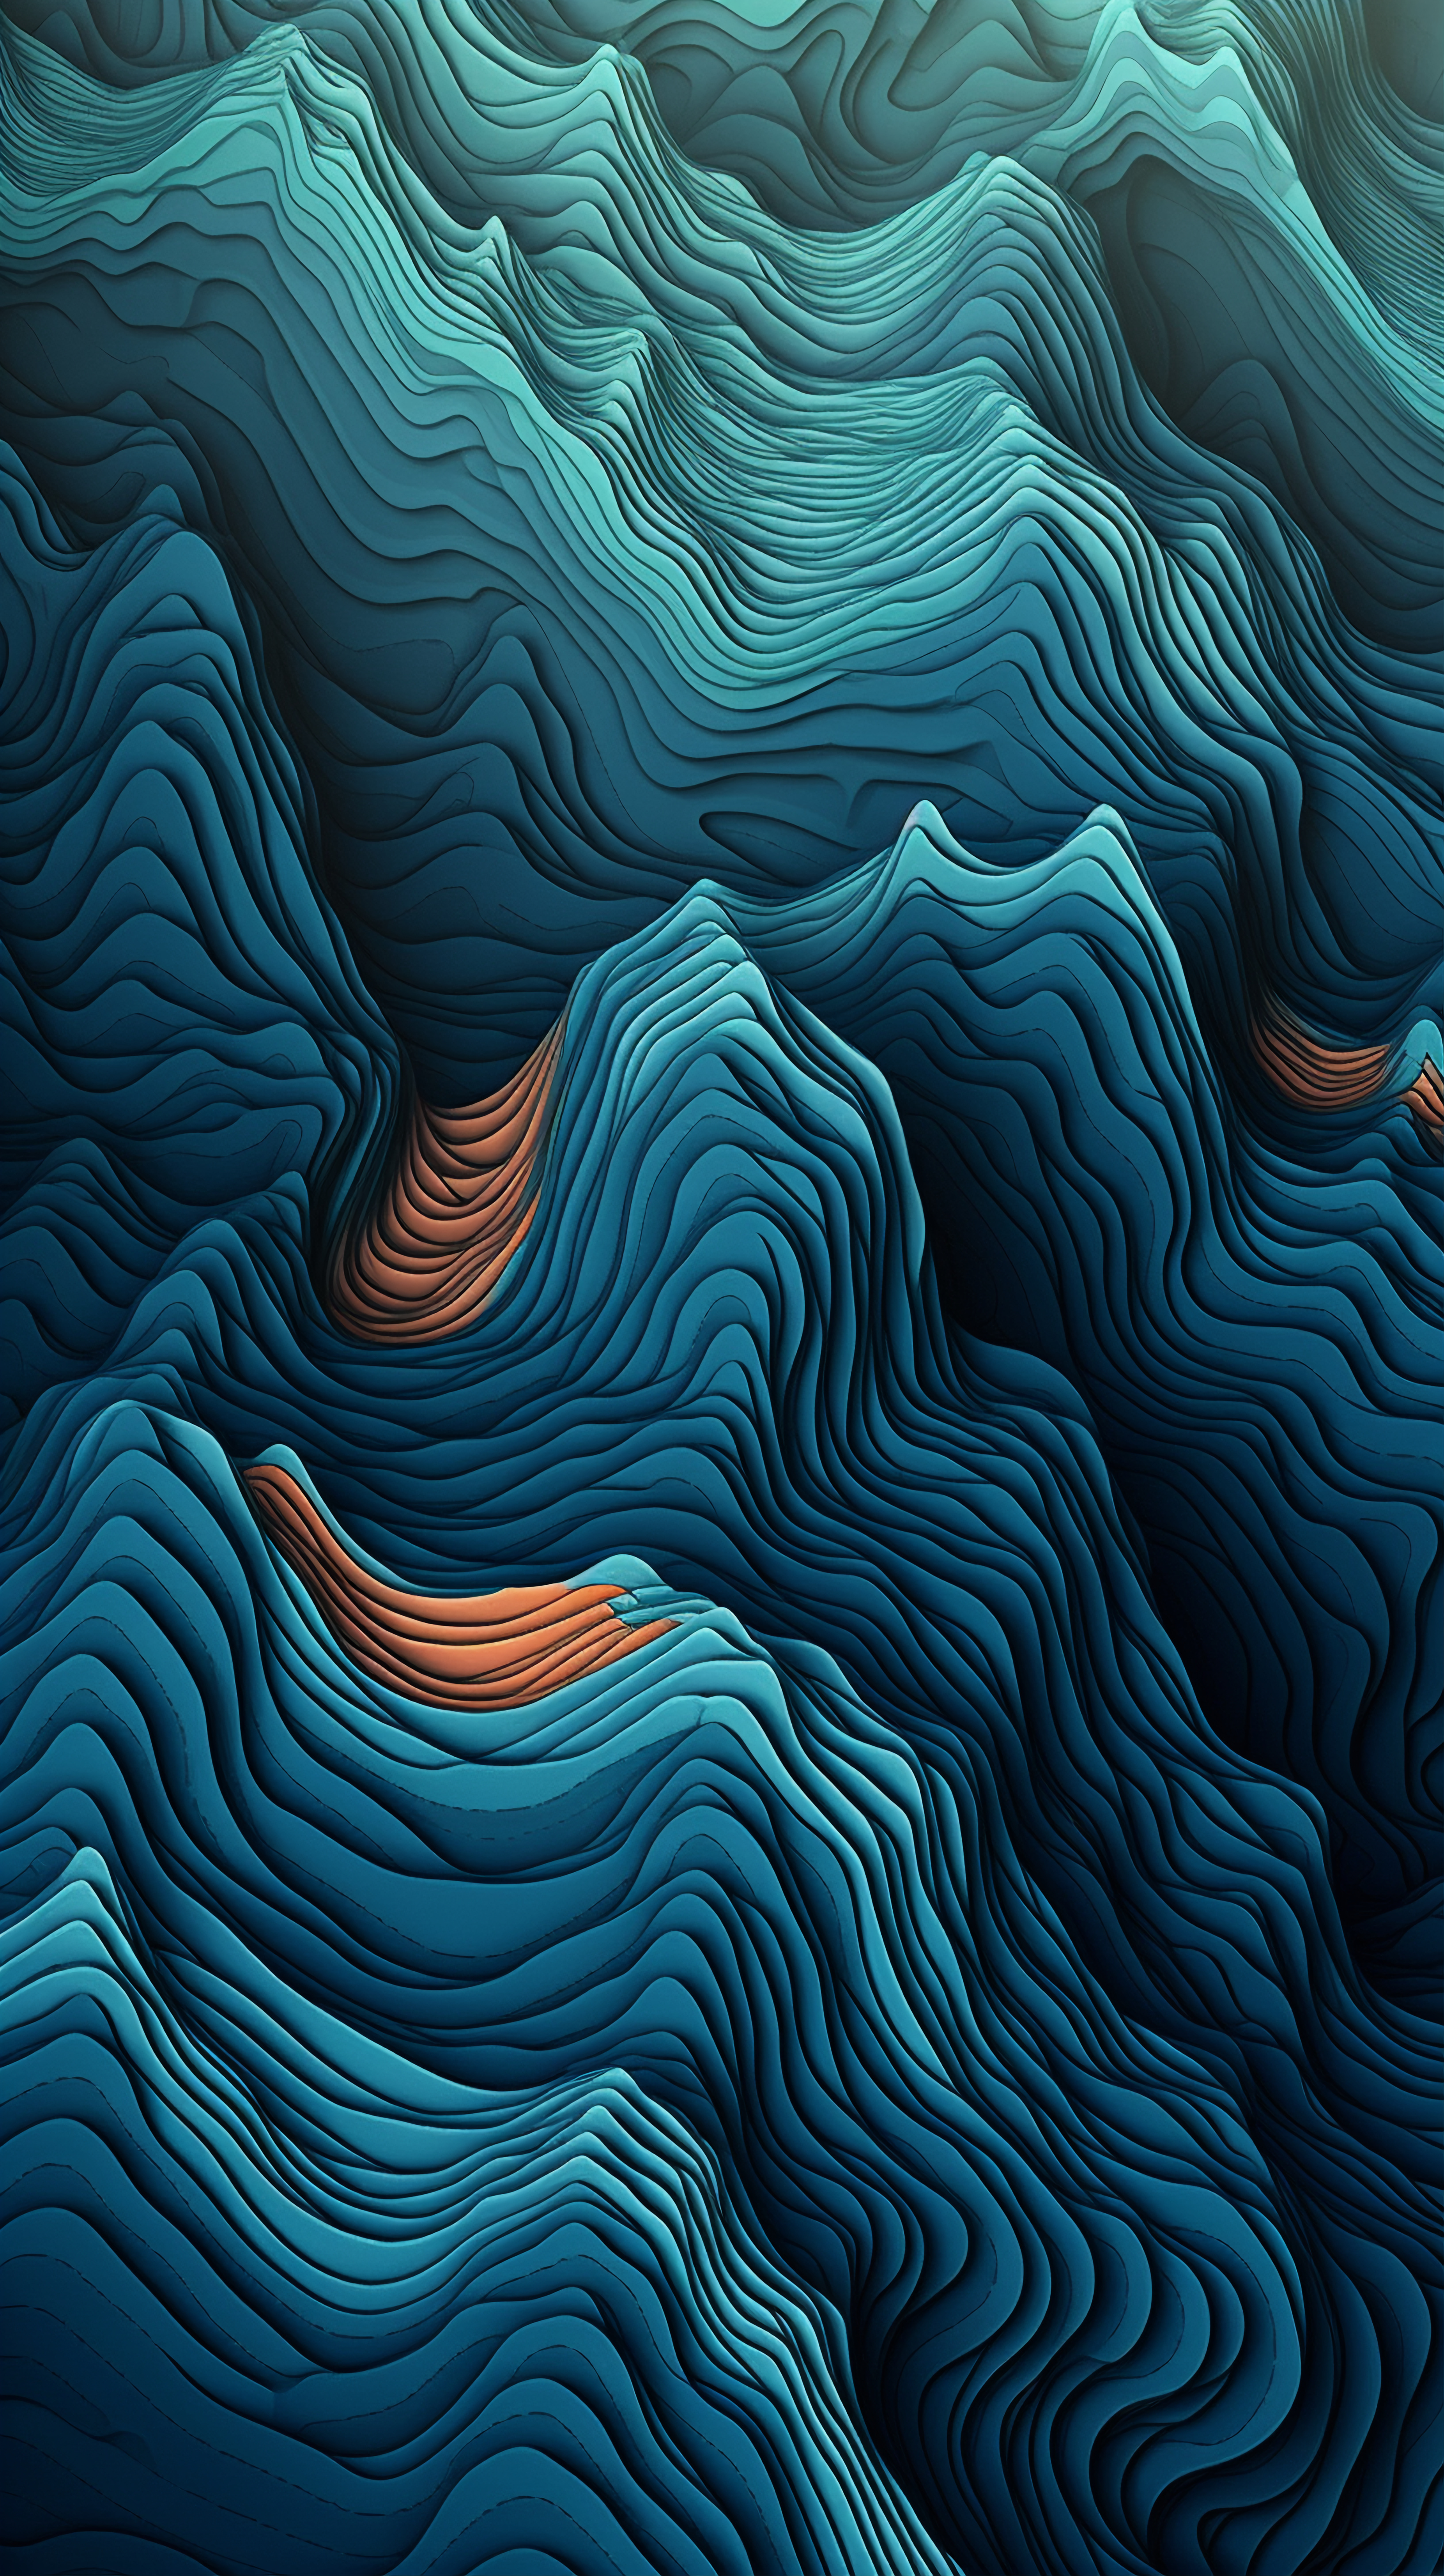
\includegraphics[angle=0,height=\paperheight]{Images/output}};
	}
\end{tikzpicture}

\vspace{7cm}

\heading{Manifolds}


%\begin{figure}[h!]
%	\centering
%	\includegraphics[width=1\linewidth]{Images/realAnalysis}
%	\caption*{$\mathbb{R}$eal Analysis, Created by DALL-E!}
%	\label{fig:realanalysis}
%	
%\end{figure}




\tableofcontents

\chapter{Euclidean Spaces}

\section{Basic Notions and Definitions}

Here in this chapter I will be covering the details of some notions that was challenging for me do digest in the first read.


\begin{definition}[Axioms of Group]
	Group is a set $ A $ along with a binary operation $ *: A\times A \to A $ that satisfies the following properties. Let $ a,b,c \in A $, then
	\begin{itemize}
		\item \textbf{Associativity}: $ a*(b*c) = (a*b)*c $.
		\item \textbf{Identity element}: $ \exists 1 \in A $ such that 
		\[ 1*a = a*1 = a. \]
		\item \textbf{Inverse element}: $ \forall a \in A\ \exists\hat{a}\in A $ such that 
		\[ a*\hat{a} = \hat{a}*a = 1. \]
	\end{itemize}
\end{definition}
\begin{remark}
	A set along with a binary operation that does not satisfy any properties is called a \textbf{magma}. If the binary operation is only associative, then we are dealing with \textbf{semi-group}. If the binary operation has an identity element as well, then we call this algebraic structure as \textbf{monoid}.
\end{remark}

\begin{definition}[Axioms of Ring]
	A ring is a set $ R $ along with two operations $ +: R\times R \to R $ and $ *: R\times R \to R $, where
	\begin{itemize}
		\item $ (R,+) $ is an Abelian group.
		\item $ (R,*) $ is a monoid.
		\item The operator $ (*) $ has distributive (left and right) law over $ (+) $ i.e.
  			\[a*(b+c) = (a*b)+(a*c), \qquad (b+c)*a = (b*a) + (c*a).\].
	\end{itemize}
\end{definition}

\begin{remark}
	\textbf{Field} is a ring where every non-zero element (i.e. inverse element in the $ (R,+) $ group in the ring) has a multiplicative inverse.
\end{remark}

\begin{definition}[Axioms of Module]
	A \textbf{module} is a group $ M $ along with a ring $ R $ where the monoid of the ring acts on $ M $ (through scalar multiplication) (i.e. it satisfies the idenity and compatibility properties) and satisfies the distributive property. I.e.
	\begin{itemize}
		\item \textbf{Compatibility of the monoid action}: $ a,b \in R,\ u \in M $ then 
		\[ a(bu) = (ab)u. \]
		\item \textbf{Identity of the monoid action}: Let $ 1 $ be the identity element of the ring $ R $. Then $ \forall u \in M $
		\[1u = u1 = u. \]
		\item \textbf{Distribution law}: $ a,b \in R $ and $ u,v \in M $ then
		\begin{itemize}
			\item $ (a+b)u = au + bu $.
			\item $ a(u+v) = au + av $.
		\end{itemize}
	\end{itemize}
\end{definition}
\begin{remark}
	A module $ (M,R) $ is called a \textbf{vector space}, if the \textbf{ring} $ R $ is a \textbf{field}.
\end{remark}

\begin{definition}[Axioms of Algebra]
	\label{def:algebra}
	An Algebra over field $ F $ is a ring $ A $ that $ F $ acts on it (thus $ A $ has vector space structure as well), where the monoid operation of $ F $ (i.e. multiplication) satisfies the homogeneity property. I.e. for $ r \in F $ and $ u,v \in A $ we have
	\[ r(uv) = (ru)v = u (rv). \]
\end{definition}

There are some important observations when combining different algebraic structures with each other to get a new one. The first is that when we combine two structures with different operators, then the operators need to satisfy the distributive laws. Also, note that when an algebraic structure (like group or monoid) acts on another algebraic structure, we need to have the identity and and compatibility conditions satisfied.

The following diagram shows how different algebraic structures are combined with each other to produce another structure.

\begin{figure}[h!]
	\centering
	\includegraphics[scale=0.5]{Images/algebraicStructures.pdf}
\end{figure}
\FloatBarrier
Note that in the figure above, I have used some non-standard notations to make the figure concise. For instance, the expression ``\textbf{$ R_{\text{mon}} @ M \ \text{with $\cdot$}$}'' means that the monoid structure in the field $ R $ acts on the group $ M $ with the ($ \cdot $) symbol. Or the expression ``\textbf{$ \times $ in $ M_{\text{mon}} $ satisfies homogen cond.}'' means the multiplication operation of the monoid structure inside the ring $ M $ satisfies the homogeneity condition (see the definition of the algebra in \autoref{def:algebra} ). Finally, $ M_{g} $ means the group structure inside the ring $ M $.

\chapter{Manifolds}

\begin{quote}
	{\color{orange} \textbf{Very important note:}} Throughout this text, to avoid repeating some words like \emph{smooth,  and etc}, we often omit them and we let the context to reflect these notions. So we emphasis that throughout this text, unless otherwise specified, by a \textbf{manifold} we always mean a $ C^\infty $ manifold. An atlas of a chart on a smooth manifold means an atlas or a chart contained in the differentiable structure of the smooth manifold.
\end{quote} 


\section{Topological manifolds and Smooth manifolds}

We start with the definition of topological manifolds. We will later study the smooth manifolds that are of our main interest in this lecture. But first, we need to review some basic definition.

\begin{definition}[Hausdorff topological space]
	A set $ A $, along with a collection of subsets of $ A $ called $ \mathcal{T} \subset 2^A $, i.e. $ (A,\mathcal{T}) $ is called a topological space if we have
	\begin{enumerate}[(I)]
		\item $ \emptyset \in \mathcal{T} $ and $ A \in \mathcal{T} $.
		\item For any infinite collection $ \set{A_\alpha}_\alpha \subset \mathcal{T} $ we have
		\[ \bigcup_{\alpha} A_\alpha \in \mathcal{T}. \]
		\item For a finite collection $ \set{A_i}_{i \in I} $ where $ I = \set{1,2,\cdots,N} $ for some $ N \in \N $, we have
		\[ \bigcap_{i \in I} A_i \in \mathcal{T}. \]
		\item $ \forall x,y \in A $ there exists $ U,V \in \mathcal{T} $ such that $ x\in U $ and $ y \in V $ and we have $ U \cap V = \emptyset $.
	\end{enumerate}
\end{definition}


The following definition reviews the notion of second countable topological spaces.

\begin{definition}[Second countable topological spaces]
	Let $ (X,\mathcal{T}) $ be a topological space. This space is second countable if there exists an at most countable collection of sets $ \mathcal{B} \subset \mathcal{T} $ such that $ \forall U \in \mathcal{T} $ we have
	\[ U = \bigcup_{A \in \mathcal{B}} A. \]
	I.e. any open set in $ \mathcal{T} $ can be written as a union of sets in $ \mathcal{B} $
\end{definition} 

The last piece of definition that we need is the notion of locally Euclidean spaces.

\begin{definition}[Locally Euclidean topological spaces]
	Let $ (X,\mathcal{T}) $ be a topological space. We say $ X $ is locally Euclidean if $ \forall p \in X $, there exists an open neighborhood $ p \in U \in \mathcal{T}$ such that is homeomorphic to an \emph{open} subset of $ \R^n $. I.e. there is a homeomorphism $ \phi: U \to \R^n $. We call the pair $ (U,\phi:U\to\R^n) $ a \emph{chart}, $ U $ a \emph{coordinate neighborhood} or a \textbf{coordinate open set}, and $ \phi $ a \emph{coordinate map} or \emph{coordinate system} on $ U $. 
\end{definition}


\begin{definition}[Topological manifolds]
	A topological manifold is a Hausdorff, second countable topological space that is locally Euclidean space. It is said to be of dimension $ n $, if it is locally Euclidean of dimension $ n $.
\end{definition}


In the following section, we will review the notion of compatible charts which will be central to our study of manifolds. Assume we have two charts $ (U,\phi) $ and $ (V,\psi) $. Since $  U,V $ are open in $ M $ (the manifold), then $ U\cap V $ is open in $ U $ and $ V $. Furthermore, since $ \phi $ is a homeomorphism to an open subset of $ \R^n $ then $ \phi(U\cap V) $ and $ \psi(U\cap V) $ are also open. One way to show this, let $ \phi(U cap V) = B, \phi(U) = A, $ and $ A\backslash B = C $. We know that $  A $ is open, and $ B\cup C = A, B \cap C = \emptyset $. Then $ A $ being open implies $ B $ and $ C $ is open. Now we can make the following definition for $ C^\infty $-compatible maps.

\begin{definition}[$ C^\infty $ compatible maps]
	Let $ M $ be a topological manifold, where $ (U,\phi) $ and $ (V,\psi) $ are two charts. These charts are called $ C^\infty $-compatible if the maps
	\[ \phi\circ \inv{\psi} : \psi(U\cap V) \to \phi(U\cap V)\qquad \text{and} \qquad  \psi \circ\inv{\phi}: \phi(U \cap V) \to \psi(U\cap V),  \]
	are $ C^\infty $. These two maps are called \emph{transition functions} between charts. 
\end{definition}

\begin{remark}
	If two $ U,V $ in the definition above, i.e. $ U\cap V = \emptyset $, then they are automatically compatible.
\end{remark}

\begin{definition}[$ C^\infty $ atlas]
	Let $ M $ be a topological manifold. The collection of charts $ \mathcal{U} = \set{(U_\alpha, \phi_\alpha)} $ is called a $ C^\infty $ atlas, or simply an atlas if 
	\begin{itemize}
		\item all of the charts are pairwise $ C^\infty $ compatible,
		\item the charts cover the whole manifold, i.e. $ M = \bigcup_\alpha U_\alpha $.
	\end{itemize}
\end{definition}

\begin{lemma}
	Let $ \mathcal{A} = \set{(U_\alpha,\phi_\alpha)}_{\alpha \in I} $ be an atlas for the manifold $ M $. Let $ (V,\psi) $ and $ (W,\sigma) $ be two charts where both of them are compatible with the atlas $ \mathcal{A} $. Then these two charts are compatible with each other.
\end{lemma}

\begin{proof}
	We start by showing that $ \psi\circ \inv{\sigma} $ is $ C^\infty $ on $ V\cap W $. Let $ p \in V \cap W $. Then $ \exists \alpha \in I $ such that $ p \in U_\alpha $ for the chart $ (U_\alpha,\phi_\alpha) $. Then 
	\[ (\psi \circ \inv{\phi_\alpha})\circ (\phi_\alpha \circ \inv{\sigma}): \sigma(W\cap U_\alpha \cap V) \to \psi(W \cap U_\alpha \cap V) \]
	is $ C^\infty $ in $ \sigma(W\cap U_\alpha \cap V) $, because it is the composition of $ C^\infty $ maps. Call $ \mathbb{B}_\alpha  = W\cap U_\alpha \cap V $. Then what we have shows is simply $ \forall p \in V \cap W $, there exists an open set $ p \in \mathbb{B}_\alpha \subset V\cap W $ for $  \alpha \in I $ and the map $ \psi \circ \inv{\sigma}  $ is $ C^\infty $ in $ \mathbb{B}_\alpha $. Since this holds for every $ p \in V \cap W $ this proves that $ \psi\circ \inv{\sigma} $ is $ C^\infty $ on $ \sigma (V\cap W) $. Similarly, we can show $ \sigma \circ \inv{\psi} $ is $ C^\infty $ on $ \psi(V\cap W) $, and this completes the proof.
\end{proof}

\begin{remark}
	Note that in an equality like $ \psi \circ \inv{\sigma} =(\psi \circ \inv{\phi_\alpha})\circ (\phi_\alpha \circ \inv{\sigma}) $, two functions in the sides of the equality have different domains. So the equality sign here means that these two functions are equal on their common domain.
\end{remark}


\begin{definition}[Maximal atlas]
	Let $ \mathcal{U} $ be an atlas for the manifold $ M $. Then $ \mathcal{U} $ is called maximal if it contains any other atlas of the manifold $ M $. Or equivalently, if $ \mathcal{M} $ is any other atlas containing $ \mathcal{U} $ then $ \mathcal{U} = \mathcal{M} $.
\end{definition}

We can use the notion of the maximal atlas to define a smooth manifold.

\begin{definition}[Smooth manifold]
	A topological manifold together with a maximal atlas is called a smooth manifold. The maximal atlas is also called a differentiable structure on $ M $.
\end{definition}


In practice, to show that a topological manifold is smooth, it is not necessary to exhibit a maximal atlas. Existence of any atlas will do so, as proposed by the following proposition.


\begin{proposition}
	Any atlas of a locally euclidean space is contained in a \emph{unique} maximal atlas.
\end{proposition}

\begin{proof}
	Let $ \frak{U} = \set{(U_\alpha, \phi_\alpha)} $ be any atlas for the locally Euclidean space $ M $. Let $ S = \set{(V_i, \psi_i)} $ denote the set of all charts compatible with $ \frak{U} $. Construct the set $ \frak{M} = \frak{U} \cup S $. We claim that this set is a maximal atlas. Let $ (W,\psi) $ be a chart compatible with $ \frak{M} $. Then it should also be compatible with $ \frak{U} $, thus it is contained in the set $ S $, i.e. $ (W,\psi) \in S $, thus in $ \frak{M} $. This shows that the atlas $ \frak{M} $ is maximal.
	
	To show the uniqueness, let $ \frak{M}' $ be another maximal atlas. Since $ \frak{M}' $ is compatible with $ \frak{U} $, thus it is also compatible with $ \frak{M} $. But due to the construction it is contained in the new atlas, thus $ \frak{M}' \subset \frak{M} $. Thus the maximal atlas is unique.
\end{proof}

Considering the proposition above, we arrive at the following important observation.

\begin{observation}[Showing a space is an smooth manifold]
	To show that a space is an smooth manifold, we just need to show that the space is
	\begin{itemize}
		\item a Hausdorff topological space that is also second countable,
		\item there exists any $ C^\infty $ atlas (not necessarily maximal).
	\end{itemize}
\end{observation}


\section{Smooth maps on a manifold}
In this section, we will study the notion of smooth maps between manifolds. We will use the notion of coordinate charts to transfer the notion of smooth maps from Euclidean spaces to manifolds. We start with the functions on manifolds.

\begin{definition}[Smooth functions on manifolds]
	Let $ f:M \to R $ be a function on a manifold. The function $ f $ is smooth at point $ p \in M $ if there exists a chart $ (U,\phi) $ such that $ p \in U $ and the map
	\[ f \circ \inv{\phi}\ :\ \phi(U) \to \R \]
	is smooth at $ p $. The function $ f $ is said to be $ C^\infty $ on $ M $ if it is $ C^\infty $ at every point of $ M $.
\end{definition}
\begin{remark} 
	Note that the smoothness of the function $ f $ in the definition above is independent of the local chart $ (U,\psi) $ that we choose. Let $ (V,\psi) $ be another local chart containing the point $ p $. Then the map $ f \circ \inv{\psi} $ is also smooth at $ p $. Because
	\[ f \circ \inv{\psi}: (f\circ \inv{\phi}) \circ (\phi \circ \inv{\psi}). \]
	We know that the map $ (\phi \circ \inv{\psi} $ is smooth at $ p $ (since the local charts in an atlas are compatible). Also $ (f\circ \inv{\phi}) $ is smooth (we have assumed so). Thus $ f \circ \inv{\psi} $ is smooth.
\end{remark}

\begin{proposition}[Smoothness of real valued functions]
	Let $ M $ be a manifold of dimension $ n $ with atlas $ \frak{U} $, and let $ f: M \to \R $ a real-valued function on $ M $. The following are equivalent:
	\begin{enumerate}[(i)]
		\item The function $ f : M \to \R $ is $ C^\infty $.
		\item The manifold $ M $ has an atlas such that for every chart $ (U,\phi) $ in the atlas, $ f\circ \inv{\phi}: \phi(U) \to \R$ is $ C^\infty $.
		\item For every chart $ (V,\psi) $ on $ M $, the function $ f\circ \inv{\psi}: \psi(V) \to \R $ is $ C^\infty $.
	\end{enumerate}
\end{proposition}

\begin{proof}
	We prove a cyclic chain of implications $ (ii)\implies (i) \implies (iii) \implies (ii) $.
	
	\noindent $ (ii) \implies (i) $: Let $ p \in M $. From the assumption we know that there is an atlas with the desired property. Thus $ \exists (U_\alpha,\phi_\alpha)  $ that contains $ p $ and the function $ f\circ\inv{\phi}: \phi(U) \to \R $ is smooth. 
	Thus $ f:M\to \R $ is smooth at $ p $, ans since the point $ p $ was arbitrary, then $ f $ is smooth on $ M $.
	
	\noindent $ (i) \implies (iii) $: Let $ p \in U $. From assumption we know that there is a coordinate open set $ U_\alpha $ such that $ f \circ \inv{\phi_\alpha}: \phi_\alpha(U)\to \R $ is smooth. Then we can write
	\[ f\circ\inv{\psi} = (f\circ\inv{\phi_\alpha})\circ(\phi_\alpha \circ \inv{\psi}) \]
	which shows that $ f\circ\inv{\psi}  $ is smooth (look at the remark below).
	
	\noindent $ (iii) \implies (ii) $: This follows immediately from the definition.
\end{proof}

%\begin{quote}
%	{\color{orange} I am not sure about the remark below. I need to discuss this with Ata in one of our weekly meetings$\ \Downarrow\Downarrow\Downarrow\Downarrow$.}
%\end{quote}
%\begin{remark}
%	Note that when we are saying ``let $ M $ be a manifold of dimension $ n $'' (in the first part of the proposition), what we really means is that the set $ M $ along with the collection of compatible charts (i.e. atlas) $ \frak{U} $ forms a manifold. In the part (iii) of the proposition above, when we say ``for every chart $ (V,\phi) $'' on manifold $ M $, what we really mean is $ (V,\phi) $ is compatible with $ \frak{U} $.
%\end{remark}

\begin{remark}
	Considering the ``very important note'' at the beginning of this chapter, we need to emphasis again that in part $ (iii) $, when we say \emph{for every chart $ (V,\psi) $ on $ M $}, we mean a chart in the unique differentiable structure of the manifold that contains the atlas $ \frak{U} $.
\end{remark}

\begin{observation}[From W. Tu]
	The smoothness conditions from the proposition above will be a recurrent motif through out the book. To prove the smoothness of an object, it is sufficient that a smoothness criterion hold on the charts of some atlas. Once the object is shown to be smooth, it then follows that the same smoothness criterion holds on every chart on the manifold.
\end{observation}


\begin{definition}[Pull back of a function]
	Let $ F: N\to M $ be a a map between manifolds, and $ \phi: M \to \R $. Then the pullback of the function $ \phi $ by $ F $ is denoted by $ F*\phi $ is defined as 
	\[ F^* \phi = \phi\circ F. \]
\end{definition}

\begin{remark}
	In this terminology, a function $ f:M \to \R $ is smooth on a chart $ (U,\phi) $ if and only if the pullback $ (\inv{\phi})^* f$ is smooth on the subset $ \phi(U) $ of Euclidean space.
\end{remark}

\subsection{Smooth maps between manifolds}
Here in this section we will discuss the smooth maps between manifolds. We will be able to recover the definition of the smooth functions on manifolds as a special case. 

\begin{definition}[Smooth maps between manifolds]
	Let $ M, N $ be manifolds with dimensions $ m,n $ respectively. A map $ F: M \to N $ is said to be smooth at point $ p \in M $, if there exists charts $ (U,\phi) $ and $ (V,\psi) $ such that $ p \in U $ and $ F(p) \in V $, and the function 
	\[ \psi\circ F \circ \inv{\phi}: \R^m \supset \phi(\inv{F}(V) \cup U) \to \R^n  \]
	is smooth at $ p $. The map $ F $ is said to be smooth on manifold $ M $ if it is smooth at every point of the manifold.
\end{definition}
\begin{remark}
	The following figure helps to digest the definition above.
	\begin{figure}[h!]
	\centering
	
	
	
	
	
	\tikzset{every picture/.style={line width=0.75pt}} %set default line width to 0.75pt        
	
	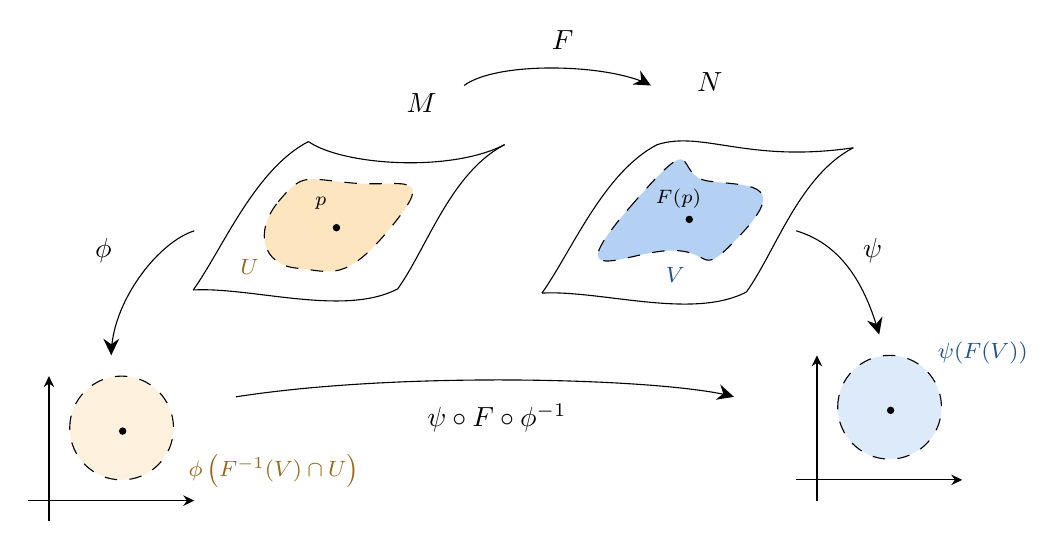
\begin{tikzpicture}[x=0.75pt,y=0.75pt,yscale=-1,xscale=1]
		%uncomment if require: \path (0,300); %set diagram left start at 0, and has height of 300
		
		%Curve Lines [id:da11806081372332144] 
		\draw    (179.5,178.5) .. controls (193.5,159) and (209,120.5) .. (235,107) ;
		%Curve Lines [id:da18965221151827483] 
		\draw    (179.5,178.5) .. controls (208,177) and (252,191.5) .. (278,178) ;
		%Curve Lines [id:da4778597706036809] 
		\draw    (278,178) .. controls (292,158.5) and (303.5,122) .. (329.5,108.5) ;
		%Curve Lines [id:da40033578881982557] 
		\draw    (235,107) .. controls (251.5,118.5) and (303.5,122) .. (329.5,108.5) ;
		%Curve Lines [id:da8289769291382043] 
		\draw    (347.5,180) .. controls (361.5,160.5) and (377,122) .. (403,108.5) ;
		%Curve Lines [id:da562782587348567] 
		\draw    (347.5,180) .. controls (376,178.5) and (420,193) .. (446,179.5) ;
		%Curve Lines [id:da8325596531064072] 
		\draw    (446,179.5) .. controls (460,160) and (471.5,123.5) .. (497.5,110) ;
		%Curve Lines [id:da2852542457229288] 
		\draw    (403,108.5) .. controls (425,101.5) and (446.5,117.5) .. (497.5,110) ;
		%Shape: Polygon Curved [id:ds40810252904164956] 
		\draw  [fill={rgb, 255:red, 245; green, 166; blue, 35 }  ,fill opacity=0.29 ][dash pattern={on 4.5pt off 4.5pt}] (220.5,136) .. controls (232.5,121.5) and (233.5,125) .. (256.5,127) .. controls (279.5,129) and (297.5,120.5) .. (275,148) .. controls (252.5,175.5) and (246,169.5) .. (229.5,168) .. controls (213,166.5) and (208.5,150.5) .. (220.5,136) -- cycle ;
		%Shape: Polygon Curved [id:ds4832622018481927] 
		\draw  [fill={rgb, 255:red, 74; green, 144; blue, 226 }  ,fill opacity=0.41 ][dash pattern={on 4.5pt off 4.5pt}] (390,138.5) .. controls (425.5,97.5) and (410,123.5) .. (427.5,126) .. controls (445,128.5) and (467,126) .. (444.5,150.5) .. controls (422,175) and (431,159) .. (409.5,159.5) .. controls (388,160) and (354.5,179.5) .. (390,138.5) -- cycle ;
		%Straight Lines [id:da8425805433734557] 
		\draw    (110,223) -- (110,290) ;
		\draw [shift={(110,220)}, rotate = 90] [fill={rgb, 255:red, 0; green, 0; blue, 0 }  ][line width=0.08]  [draw opacity=0] (5.36,-2.57) -- (0,0) -- (5.36,2.57) -- (3.56,0) -- cycle    ;
		%Straight Lines [id:da3867027047624212] 
		\draw    (177,280) -- (100,280) ;
		\draw [shift={(180,280)}, rotate = 180] [fill={rgb, 255:red, 0; green, 0; blue, 0 }  ][line width=0.08]  [draw opacity=0] (5.36,-2.57) -- (0,0) -- (5.36,2.57) -- (3.56,0) -- cycle    ;
		%Shape: Circle [id:dp9021706695013989] 
		\draw  [fill={rgb, 255:red, 245; green, 166; blue, 35 }  ,fill opacity=0.15 ][dash pattern={on 4.5pt off 4.5pt}] (120,245) .. controls (120,231.19) and (131.19,220) .. (145,220) .. controls (158.81,220) and (170,231.19) .. (170,245) .. controls (170,258.81) and (158.81,270) .. (145,270) .. controls (131.19,270) and (120,258.81) .. (120,245) -- cycle ;
		%Straight Lines [id:da20897051537256983] 
		\draw    (480,213) -- (480,280) ;
		\draw [shift={(480,210)}, rotate = 90] [fill={rgb, 255:red, 0; green, 0; blue, 0 }  ][line width=0.08]  [draw opacity=0] (5.36,-2.57) -- (0,0) -- (5.36,2.57) -- (3.56,0) -- cycle    ;
		%Straight Lines [id:da4413765041127402] 
		\draw    (547,270) -- (470,270) ;
		\draw [shift={(550,270)}, rotate = 180] [fill={rgb, 255:red, 0; green, 0; blue, 0 }  ][line width=0.08]  [draw opacity=0] (5.36,-2.57) -- (0,0) -- (5.36,2.57) -- (3.56,0) -- cycle    ;
		%Shape: Circle [id:dp2483574720488635] 
		\draw  [fill={rgb, 255:red, 74; green, 144; blue, 226 }  ,fill opacity=0.19 ][dash pattern={on 4.5pt off 4.5pt}] (490,235) .. controls (490,221.19) and (501.19,210) .. (515,210) .. controls (528.81,210) and (540,221.19) .. (540,235) .. controls (540,248.81) and (528.81,260) .. (515,260) .. controls (501.19,260) and (490,248.81) .. (490,235) -- cycle ;
		%Curve Lines [id:da8553312339361681] 
		\draw    (310,80) .. controls (325.36,68.48) and (376.66,69.4) .. (397.55,78.78) ;
		\draw [shift={(400,80)}, rotate = 208.93] [fill={rgb, 255:red, 0; green, 0; blue, 0 }  ][line width=0.08]  [draw opacity=0] (8.04,-3.86) -- (0,0) -- (8.04,3.86) -- (5.34,0) -- cycle    ;
		%Curve Lines [id:da778090429217146] 
		\draw    (470,150) .. controls (490.75,156.27) and (502.18,173.72) .. (509.25,197.4) ;
		\draw [shift={(510,200)}, rotate = 254.36] [fill={rgb, 255:red, 0; green, 0; blue, 0 }  ][line width=0.08]  [draw opacity=0] (8.04,-3.86) -- (0,0) -- (8.04,3.86) -- (5.34,0) -- cycle    ;
		%Curve Lines [id:da210913418624189] 
		\draw    (180,150) .. controls (163.11,155.31) and (141.57,182.5) .. (140.08,207.31) ;
		\draw [shift={(140,210)}, rotate = 270] [fill={rgb, 255:red, 0; green, 0; blue, 0 }  ][line width=0.08]  [draw opacity=0] (8.04,-3.86) -- (0,0) -- (8.04,3.86) -- (5.34,0) -- cycle    ;
		%Curve Lines [id:da8925336292700183] 
		\draw    (200,230) .. controls (281,217.39) and (403.86,221.25) .. (437.17,229.25) ;
		\draw [shift={(440,230)}, rotate = 196.61] [fill={rgb, 255:red, 0; green, 0; blue, 0 }  ][line width=0.08]  [draw opacity=0] (8.04,-3.86) -- (0,0) -- (8.04,3.86) -- (5.34,0) -- cycle    ;
		%Shape: Circle [id:dp7473837647062398] 
		\draw  [fill={rgb, 255:red, 0; green, 0; blue, 0 }  ,fill opacity=1 ] (247,148.5) .. controls (247,147.67) and (247.67,147) .. (248.5,147) .. controls (249.33,147) and (250,147.67) .. (250,148.5) .. controls (250,149.33) and (249.33,150) .. (248.5,150) .. controls (247.67,150) and (247,149.33) .. (247,148.5) -- cycle ;
		%Shape: Circle [id:dp9244279482747275] 
		\draw  [fill={rgb, 255:red, 0; green, 0; blue, 0 }  ,fill opacity=1 ] (417,144.5) .. controls (417,143.67) and (417.67,143) .. (418.5,143) .. controls (419.33,143) and (420,143.67) .. (420,144.5) .. controls (420,145.33) and (419.33,146) .. (418.5,146) .. controls (417.67,146) and (417,145.33) .. (417,144.5) -- cycle ;
		%Shape: Circle [id:dp5699925804076371] 
		\draw  [fill={rgb, 255:red, 0; green, 0; blue, 0 }  ,fill opacity=1 ] (144,246.5) .. controls (144,245.67) and (144.67,245) .. (145.5,245) .. controls (146.33,245) and (147,245.67) .. (147,246.5) .. controls (147,247.33) and (146.33,248) .. (145.5,248) .. controls (144.67,248) and (144,247.33) .. (144,246.5) -- cycle ;
		%Shape: Circle [id:dp11209906657188418] 
		\draw  [fill={rgb, 255:red, 0; green, 0; blue, 0 }  ,fill opacity=1 ] (514,236.5) .. controls (514,235.67) and (514.67,235) .. (515.5,235) .. controls (516.33,235) and (517,235.67) .. (517,236.5) .. controls (517,237.33) and (516.33,238) .. (515.5,238) .. controls (514.67,238) and (514,237.33) .. (514,236.5) -- cycle ;
		
		% Text Node
		\draw (281,82.4) node [anchor=north west][inner sep=0.75pt]    {$M$};
		% Text Node
		\draw (421,72.4) node [anchor=north west][inner sep=0.75pt]    {$N$};
		% Text Node
		\draw (351,52.4) node [anchor=north west][inner sep=0.75pt]    {$F$};
		% Text Node
		\draw (501,152.4) node [anchor=north west][inner sep=0.75pt]    {$\psi $};
		% Text Node
		\draw (131,152.4) node [anchor=north west][inner sep=0.75pt]    {$\phi $};
		% Text Node
		\draw (291,232.4) node [anchor=north west][inner sep=0.75pt]    {$\psi \circ F\circ \phi ^{-1}$};
		% Text Node
		\draw (237,132.4) node [anchor=north west][inner sep=0.75pt]  [font=\scriptsize]  {$p$};
		% Text Node
		\draw (401,128.4) node [anchor=north west][inner sep=0.75pt]  [font=\scriptsize]  {$F( p)$};
		% Text Node
		\draw (201,162.4) node [anchor=north west][inner sep=0.75pt]  [font=\footnotesize,color={rgb, 255:red, 155; green, 104; blue, 25 }  ,opacity=1 ]  {$U$};
		% Text Node
		\draw (406,166.4) node [anchor=north west][inner sep=0.75pt]  [font=\footnotesize,color={rgb, 255:red, 29; green, 81; blue, 148 }  ,opacity=1 ]  {$V$};
		% Text Node
		\draw (537,202.4) node [anchor=north west][inner sep=0.75pt]  [font=\footnotesize,color={rgb, 255:red, 29; green, 81; blue, 148 }  ,opacity=1 ]  {$\psi ( F( V))$};
		% Text Node
		\draw (176,256.4) node [anchor=north west][inner sep=0.75pt]  [font=\footnotesize,color={rgb, 255:red, 155; green, 104; blue, 25 }  ,opacity=1 ]  {$\phi \left( F^{-1}( V) \cap U\right)$};
		
		
	\end{tikzpicture}
\end{figure}
\end{remark}

\begin{remark}
	Since the Euclidean space is indeed a smooth manifolds, then we can recover the definition of smooth functions on manifolds form the definition above. Let $ M $ be a manifold, and $ N = \R^n $ with the atlas $ \set{(\R^n, \mathds{1}: \R^n \to \R^n)} $, then we will have the notion of vector valued functions on manifold. By setting $ n=1 $ we will recover the definition of smooth function on manifold.
\end{remark}

In the following proposition we will be showing that the smoothness of the map is independent of the charts chosen, thus the smoothness of the map is well-defined.

\begin{proposition}[Smoothness of maps between manifolds is well-defined]
	\label{prop:SmoothnessWellDefined}
	Suppose $ F: N \to M $ is $ C^\infty $ at $ p \in N $. If $ (U,\phi) $ is any chart in $ N $ that contains $ p $ and $ (V,\psi) $ is any chart in $ M $ that contains $ F(p) $, then $ \psi \circ F \circ \inv{\phi} $ is smooth at $ \phi(p) $.
\end{proposition}

\begin{proof}
	Since $ F: N \to M $ is smooth at $ p \in N $, then there are charts $ (G,\gamma) $ and $ (L, \lambda) $ (from the corresponding maximal atlases) such that $ p \in G \subset N $ and $ F(p) \in L \subset M $ and the function 
	\[ (\lambda \circ F \circ \inv{\gamma}): \gamma(\inv{F}(L) \cap G ) \to \lambda(F(G)) \]
	is smooth at $ p $. Consider the charts $ (U,\phi) $ and $ (V,\psi) $ as above. Then the function
	\[ \psi \circ F \circ \inv{\phi} = (\psi \circ \inv{\lambda})\circ(\lambda\circ F \circ \inv{\gamma})\circ(\gamma\circ \inv{\phi}). \]
	Note that the equality sign above merely means the functions are equal on their common domain, as the function in RHS and the function in LHS have different domains. We know that the coordinate maps $ \psi, \lambda $, and $ \gamma, \phi$ are compatible respectively. Thus the function $ \psi \circ F \circ \inv{\phi} $ is smooth at $ \phi(p) $. See the remark below for mode details.
\end{proof}

\begin{remark}
	In the proof above and in the equality 
	\[ \psi \circ F \circ \inv{\phi} = (\psi \circ \inv{\lambda})\circ(\lambda\circ F \circ \inv{\gamma})\circ(\gamma\circ \inv{\phi}) \]
	thus equality sign does not indicate that these function are equal, but it just indicates that these two functions are equal in their common domain. To be more clear, for the function in the LHS we have
	\[ \psi \circ F \circ \inv{\phi} : \phi(\inv{F}(V)\cap U) \to \psi(F(U)). \]
	But for the function in the LHS we have
	\[ (\psi \circ \inv{\lambda})\circ(\lambda\circ F \circ \inv{\gamma})\circ(\gamma\circ \inv{\phi}):
	\phi(\inv{F}(L\cap V) \cap (G\cap U)) \to \psi(F(L\cap V))
	 \]
\end{remark}

\begin{proposition}[Smoothness of maps in terms of charts]
	\label{prop:smoothnessInTermsOfCharts}
	Let $ N $ and $ M $ be smooth manifolds, and $ F: N \to M $ a continuous map. The following are equivalent:
	\begin{enumerate}[(i)]
		\item The map $ F: N\to M $ is $ C^\infty $.
		\item There are atlases $ \frak{U} $ for $ N $ and $ \frak{V} $  for $ M $ such that for every chart $ (U,\phi) $ in $ \frak{U} $ and $ (V,\psi) $ in $ \frak{V} $ the map
		\[ \psi \circ F \circ \inv{\phi}: \phi(\inv{F}(V)\cap U) \to \R^m  \]
		is $ C^\infty $.
		\item For every chart $ (U,\phi) $ on $ N $ and $ (V,\psi) $ on $ M $, the map
		\[ \psi \circ F \circ \inv{\phi}: \phi(U \cap \inv{F}(V)) \to \R^m \]
		is $ C^\infty $.
	\end{enumerate}
\end{proposition}
\begin{proof}
	We will prove this by showing a cyclic chain of implications $ (ii)\implies (i)\implies (iii)\implies (ii) $.
	\begin{itemize}
		\item $ (ii)\implies (i) $. Let $ p \in N $. Then by hypothesis there are charts $ (U,\phi) $ and $ (V,\psi) $  such that $ p \in U $ and $ F(p) \in V $ and the map 
		\[ \psi \circ F \circ \inv{\phi}: \phi(\inv{F}(V)\cap U) \to \R^m \]
		is smooth at $ \phi(p) $, thus $ F $ is smooth at $ p $. Since $ p $ is arbitrary, then $ F $ is smooth on $ N $.
		\item $ (i) \implies (iii) $. This follows immediately from \autoref{prop:SmoothnessWellDefined}.
		\item $ (iii) \implies (ii) $. Since $ N, M $ are smooth manifolds, then they have maximal atlases. Let $ \frak{U} $ be the maximal atlas for $ N $ and $ \frak{V} $ be the maximal atlas for $ M $. This $ (ii) $ follows immediately form $ (iii) $.
		
	\end{itemize}
\end{proof}

\begin{proposition}[Composition of $ C^\infty $ maps]
	If $ F:N\to M $ and $ G:M\to P $ are $ C^\infty $ maps of manifolds, then the composite $ G\circ F: N \to P $ is a smooth map.
\end{proposition}

\begin{proof}
	We will demonstrate two proofs for this proposition to demonstrate what happens if we do not notice a possible level of abstraction. The first proof below is a very crude, hard-core, direct proof, that seems to be tough and easy to make mistakes, just because it is not encapsulating some of the details into another proposition. However, for the second proof, it will encapsulate some of the details into the results of the \autoref{prop:smoothnessInTermsOfCharts}, which will allows us to do a more high level thinking.
\end{proof}




\newpage


\section{Solved Problems}

\begin{problem}[A $ C^\infty $ atlas on a circle (From W. Tu)]
	construct a $ C^\infty $ atlas for the unit circle $ S^1 $. 
\end{problem}
\begin{solution}
	The unit circle $ C^1 $ can be described as a set of points $ S^1 =  \set{e^{it}| t \in [0,2\pi]} $. Let $ U_1 $ and $ U_2 $ be two subsets of $ S^1 $ described as
	\[ U_1 = \set{e^{it}| t \in (-\pi,\pi)},\qquad U_2 = \set{e^{it}| t \in (0,2\pi)}. \]
	Consider the functions $ \phi_\alpha: U_\alpha \to \R $ for $ \alpha = 1,2 $ given by
	\begin{align*}
		&\phi_1(e^{it}) = t, \qquad -\pi<t<\pi,\\
		&\phi_2(e^{it}) = t, \qquad 0<t<2\pi.
	\end{align*}
	These functions are in fact different branches of the complex logarithm function $ 1/i\log(z) $, thus homeomorphisms onto their respective images. Thus $ \set{(U_1,\phi_1),(U_2,\phi_2)} $ is an atlas for $ S^1 $. To demonstrate the compatibility of these charts, we need to first calculate $ U_1 \cap U_2 $. This set has two connected components, i.e. $ U_1 \cap U_2 = A \sqcup B $ where $ \sqcup $ is used to demonstrate the disjoint union of $ A,B $. Explicitly, we can write
	\[ A = \set{e^{it}| t \in (-\pi,0)}, \qquad B = \set{e^{it}| t\in(0,\pi)}. \]
	First, we start with the function $ \phi_1 \circ \phi_2^{-1}: \underbrace{\phi_2(U_1\cap U_2)}_{(0,\pi)\sqcup (\pi,2\pi)} \to \underbrace{\phi_1(U_1\cap U_2)}_{(-\pi,0)\sqcup (0,\pi)} $. For this function we have
	\[ (\phi_1\circ\phi_2^{-1})(t) = \begin{cases}
		t \qquad &t\in(0,\pi),\\
		t - 2\pi \qquad &t\in(\pi,2\pi).
	\end{cases} \]
	Similarly, for $ \phi_2 \circ \phi_1^{-1}: \underbrace{\phi_1(U_1\cap U_2)}_{(-\pi,0)\sqcup (0,\pi)} \to \underbrace{\phi_2(U_1\cap U_2)}_{(0,\pi)\sqcup (\pi,2\pi)} $ we can write
	\[ (\phi_2\circ\phi_1^{-1})(t) = \begin{cases}
		t+2\pi \qquad &t\in(0,\pi),\\
		t \qquad &t\in(\pi,2\pi).
	\end{cases} \]
	\begin{figure}[h!]
	\centering

	
	
	\tikzset{every picture/.style={line width=0.75pt}} %set default line width to 0.75pt        
	
	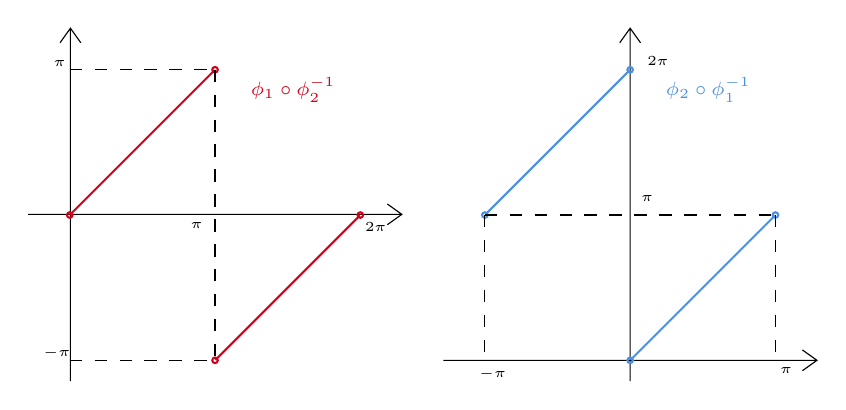
\begin{tikzpicture}[x=0.75pt,y=0.75pt,yscale=-1,xscale=1]
		%uncomment if require: \path (0,300); %set diagram left start at 0, and has height of 300
		
		%Shape: Axis 2D [id:dp031269396086308854] 
		\draw  (180,189.67) -- (360,189.67)(200.33,100) -- (200.33,270) (353,184.67) -- (360,189.67) -- (353,194.67) (195.33,107) -- (200.33,100) -- (205.33,107)  ;
		%Straight Lines [id:da8173483474090752] 
		\draw [color={rgb, 255:red, 208; green, 2; blue, 27 }  ,draw opacity=1 ][line width=0.75]    (200.24,189.76) -- (269.76,120.24) ;
		\draw [shift={(270,120)}, rotate = 315] [color={rgb, 255:red, 208; green, 2; blue, 27 }  ,draw opacity=1 ][line width=0.75]      (0, 0) circle [x radius= 1.34, y radius= 1.34]   ;
		\draw [shift={(200,190)}, rotate = 315] [color={rgb, 255:red, 208; green, 2; blue, 27 }  ,draw opacity=1 ][line width=0.75]      (0, 0) circle [x radius= 1.34, y radius= 1.34]   ;
		%Straight Lines [id:da7972743834901372] 
		\draw [color={rgb, 255:red, 208; green, 2; blue, 27 }  ,draw opacity=1 ][line width=0.75]    (270.24,259.76) -- (339.76,190.24) ;
		\draw [shift={(340,190)}, rotate = 315] [color={rgb, 255:red, 208; green, 2; blue, 27 }  ,draw opacity=1 ][line width=0.75]      (0, 0) circle [x radius= 1.34, y radius= 1.34]   ;
		\draw [shift={(270,260)}, rotate = 315] [color={rgb, 255:red, 208; green, 2; blue, 27 }  ,draw opacity=1 ][line width=0.75]      (0, 0) circle [x radius= 1.34, y radius= 1.34]   ;
		%Straight Lines [id:da11749218813373297] 
		\draw  [dash pattern={on 4.5pt off 4.5pt}]  (270,120) -- (270,260) ;
		%Shape: Axis 2D [id:dp7242837319994968] 
		\draw  (380,260) -- (560,260)(470,100) -- (470,270) (553,255) -- (560,260) -- (553,265) (465,107) -- (470,100) -- (475,107)  ;
		%Straight Lines [id:da7954245800299584] 
		\draw [color={rgb, 255:red, 74; green, 144; blue, 226 }  ,draw opacity=1 ][line width=0.75]    (400.24,189.76) -- (469.76,120.24) ;
		\draw [shift={(470,120)}, rotate = 315] [color={rgb, 255:red, 74; green, 144; blue, 226 }  ,draw opacity=1 ][line width=0.75]      (0, 0) circle [x radius= 1.34, y radius= 1.34]   ;
		\draw [shift={(400,190)}, rotate = 315] [color={rgb, 255:red, 74; green, 144; blue, 226 }  ,draw opacity=1 ][line width=0.75]      (0, 0) circle [x radius= 1.34, y radius= 1.34]   ;
		%Straight Lines [id:da15608839189923596] 
		\draw [color={rgb, 255:red, 74; green, 144; blue, 226 }  ,draw opacity=1 ][line width=0.75]    (470.24,259.76) -- (539.76,190.24) ;
		\draw [shift={(540,190)}, rotate = 315] [color={rgb, 255:red, 74; green, 144; blue, 226 }  ,draw opacity=1 ][line width=0.75]      (0, 0) circle [x radius= 1.34, y radius= 1.34]   ;
		\draw [shift={(470,260)}, rotate = 315] [color={rgb, 255:red, 74; green, 144; blue, 226 }  ,draw opacity=1 ][line width=0.75]      (0, 0) circle [x radius= 1.34, y radius= 1.34]   ;
		%Straight Lines [id:da8863860410352722] 
		\draw  [dash pattern={on 4.5pt off 4.5pt}]  (400,190) -- (400,260) ;
		%Straight Lines [id:da8092780134149673] 
		\draw  [dash pattern={on 4.5pt off 4.5pt}]  (540,190) -- (540,260) ;
		%Straight Lines [id:da9907647632614371] 
		\draw  [dash pattern={on 4.5pt off 4.5pt}]  (400,190) -- (540,190) ;
		%Straight Lines [id:da6719155425075689] 
		\draw  [dash pattern={on 4.5pt off 4.5pt}]  (200,260) -- (270,260) ;
		%Straight Lines [id:da26461137148185054] 
		\draw  [dash pattern={on 4.5pt off 4.5pt}]  (200,120) -- (270,120) ;
		
		% Text Node
		\draw (257,192.4) node [anchor=north west][inner sep=0.75pt]  [font=\tiny]  {$\pi $};
		% Text Node
		\draw (286,122.4) node [anchor=north west][inner sep=0.75pt]  [font=\scriptsize,color={rgb, 255:red, 208; green, 2; blue, 27 }  ,opacity=1 ]  {$\phi _{1} \circ \phi _{2}^{-1}$};
		% Text Node
		\draw (341,192.4) node [anchor=north west][inner sep=0.75pt]  [font=\tiny]  {$2\pi $};
		% Text Node
		\draw (396,262.4) node [anchor=north west][inner sep=0.75pt]  [font=\tiny]  {$-\pi $};
		% Text Node
		\draw (486,122.4) node [anchor=north west][inner sep=0.75pt]  [font=\scriptsize,color={rgb, 255:red, 74; green, 144; blue, 226 }  ,opacity=1 ]  {$\phi _{2} \circ \phi _{1}^{-1}$};
		% Text Node
		\draw (541,262.4) node [anchor=north west][inner sep=0.75pt]  [font=\tiny]  {$\pi $};
		% Text Node
		\draw (474,179.4) node [anchor=north west][inner sep=0.75pt]  [font=\tiny]  {$\pi $};
		% Text Node
		\draw (477,112.4) node [anchor=north west][inner sep=0.75pt]  [font=\tiny]  {$2\pi $};
		% Text Node
		\draw (191,114.4) node [anchor=north west][inner sep=0.75pt]  [font=\tiny]  {$\pi $};
		% Text Node
		\draw (186,252.4) node [anchor=north west][inner sep=0.75pt]  [font=\tiny]  {$-\pi $};
		
		
	\end{tikzpicture}
\end{figure}

\end{solution}

\begin{observation}
	I was thinking about my solution to the problem above, and I thought it is wrong, as I was thinking that the function $ \phi_1 $ is not homeomorphism as it is not continuous. But the point that I was missing is that this function is indeed continuous on its domain and the point of discontinuity (i.e. $ x = \pi $) is not in the domain. 
\end{observation}

\begin{problem}{Another $ C^\infty $ atlas on a circle}
	In the previous problem, we constructed an atlas for a unit circle siting in the complex plane. In this problem we are going to construct a different atlas for a unit circle siting in the $ x-y $ plane. The following diagram are the charts for this unit circle. Write these charts explicitly and check if they are pairwise compatible.
	\begin{figure}[h!]
	
	
	\centering
	\tikzset{every picture/.style={line width=0.75pt}} %set default line width to 0.75pt        
	
	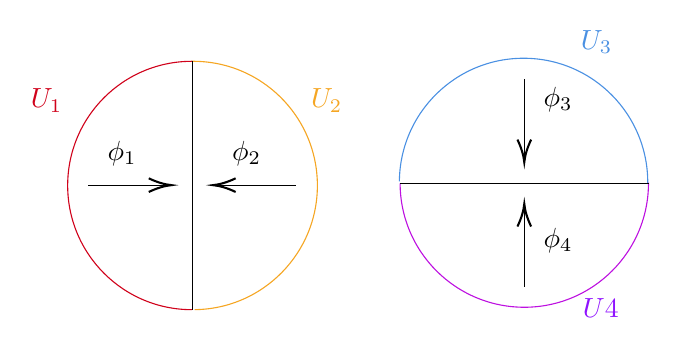
\begin{tikzpicture}[x=0.75pt,y=0.75pt,yscale=-1,xscale=1]
		%uncomment if require: \path (0,300); %set diagram left start at 0, and has height of 300
		
		%Shape: Arc [id:dp023481932229717062] 
		\draw  [draw opacity=0] (199.83,250) .. controls (199.83,250) and (199.83,250) .. (199.83,250) .. controls (199.83,250) and (199.83,250) .. (199.83,250) .. controls (166.79,250) and (140,223.21) .. (140,190.17) .. controls (140,157.12) and (166.79,130.33) .. (199.83,130.33) -- (199.83,190.17) -- cycle ; \draw  [color={rgb, 255:red, 208; green, 2; blue, 27 }  ,draw opacity=1 ] (199.83,250) .. controls (199.83,250) and (199.83,250) .. (199.83,250) .. controls (199.83,250) and (199.83,250) .. (199.83,250) .. controls (166.79,250) and (140,223.21) .. (140,190.17) .. controls (140,157.12) and (166.79,130.33) .. (199.83,130.33) ;  
		%Shape: Arc [id:dp8279857043077765] 
		\draw  [draw opacity=0] (199.83,130.33) .. controls (199.83,130.33) and (199.83,130.33) .. (199.83,130.33) .. controls (232.88,129.98) and (259.95,156.47) .. (260.31,189.52) .. controls (260.67,222.56) and (234.17,249.64) .. (201.13,249.99) -- (200.48,190.16) -- cycle ; \draw  [color={rgb, 255:red, 245; green, 166; blue, 35 }  ,draw opacity=1 ] (199.83,130.33) .. controls (199.83,130.33) and (199.83,130.33) .. (199.83,130.33) .. controls (232.88,129.98) and (259.95,156.47) .. (260.31,189.52) .. controls (260.67,222.56) and (234.17,249.64) .. (201.13,249.99) ;  
		%Shape: Arc [id:dp2277450931666709] 
		\draw  [draw opacity=0] (299.82,188.21) .. controls (299.82,188.21) and (299.82,188.21) .. (299.82,188.21) .. controls (300.08,155.16) and (327.08,128.59) .. (360.13,128.86) .. controls (393.17,129.12) and (419.75,156.12) .. (419.48,189.17) -- (359.65,188.69) -- cycle ; \draw  [color={rgb, 255:red, 74; green, 144; blue, 226 }  ,draw opacity=1 ] (299.82,188.21) .. controls (299.82,188.21) and (299.82,188.21) .. (299.82,188.21) .. controls (300.08,155.16) and (327.08,128.59) .. (360.13,128.86) .. controls (393.17,129.12) and (419.75,156.12) .. (419.48,189.17) ;  
		%Shape: Arc [id:dp16056893747855794] 
		\draw  [draw opacity=0] (419.83,188.83) .. controls (419.83,188.83) and (419.83,188.83) .. (419.83,188.83) .. controls (419.93,221.88) and (393.21,248.74) .. (360.17,248.83) .. controls (327.12,248.93) and (300.26,222.21) .. (300.17,189.17) -- (360,189) -- cycle ; \draw  [color={rgb, 255:red, 189; green, 16; blue, 224 }  ,draw opacity=1 ] (419.83,188.83) .. controls (419.83,188.83) and (419.83,188.83) .. (419.83,188.83) .. controls (419.93,221.88) and (393.21,248.74) .. (360.17,248.83) .. controls (327.12,248.93) and (300.26,222.21) .. (300.17,189.17) ;  
		%Straight Lines [id:da9947609889928073] 
		\draw    (150,190) -- (188,190) ;
		\draw [shift={(190,190)}, rotate = 180] [color={rgb, 255:red, 0; green, 0; blue, 0 }  ][line width=0.75]    (10.93,-3.29) .. controls (6.95,-1.4) and (3.31,-0.3) .. (0,0) .. controls (3.31,0.3) and (6.95,1.4) .. (10.93,3.29)   ;
		%Straight Lines [id:da6553860547904606] 
		\draw    (212,190) -- (250,190) ;
		\draw [shift={(210,190)}, rotate = 0] [color={rgb, 255:red, 0; green, 0; blue, 0 }  ][line width=0.75]    (10.93,-3.29) .. controls (6.95,-1.4) and (3.31,-0.3) .. (0,0) .. controls (3.31,0.3) and (6.95,1.4) .. (10.93,3.29)   ;
		%Straight Lines [id:da19474028508083085] 
		\draw    (360,139) -- (360,177) ;
		\draw [shift={(360,179)}, rotate = 270] [color={rgb, 255:red, 0; green, 0; blue, 0 }  ][line width=0.75]    (10.93,-3.29) .. controls (6.95,-1.4) and (3.31,-0.3) .. (0,0) .. controls (3.31,0.3) and (6.95,1.4) .. (10.93,3.29)   ;
		%Straight Lines [id:da648683487634115] 
		\draw    (360,239) -- (360,201) ;
		\draw [shift={(360,199)}, rotate = 90] [color={rgb, 255:red, 0; green, 0; blue, 0 }  ][line width=0.75]    (10.93,-3.29) .. controls (6.95,-1.4) and (3.31,-0.3) .. (0,0) .. controls (3.31,0.3) and (6.95,1.4) .. (10.93,3.29)   ;
		%Straight Lines [id:da9130830416071034] 
		\draw    (200,130) -- (200,250) ;
		%Straight Lines [id:da1322223309435544] 
		\draw    (420,189) -- (300,189) ;
		
		% Text Node
		\draw (121,142.4) node [anchor=north west][inner sep=0.75pt]  [color={rgb, 255:red, 208; green, 2; blue, 27 }  ,opacity=1 ]  {$U_{1}$};
		% Text Node
		\draw (256,142.4) node [anchor=north west][inner sep=0.75pt]  [color={rgb, 255:red, 245; green, 166; blue, 35 }  ,opacity=1 ]  {$U_{2}$};
		% Text Node
		\draw (386,114.4) node [anchor=north west][inner sep=0.75pt]  [color={rgb, 255:red, 74; green, 144; blue, 226 }  ,opacity=1 ]  {$U_{3}$};
		% Text Node
		\draw (387,243.4) node [anchor=north west][inner sep=0.75pt]  [color={rgb, 255:red, 144; green, 19; blue, 254 }  ,opacity=1 ]  {$U4$};
		% Text Node
		\draw (158,167.4) node [anchor=north west][inner sep=0.75pt]    {$\phi _{1}$};
		% Text Node
		\draw (218,167.4) node [anchor=north west][inner sep=0.75pt]    {$\phi _{2}$};
		% Text Node
		\draw (368,141.4) node [anchor=north west][inner sep=0.75pt]    {$\phi _{3}$};
		% Text Node
		\draw (368,209.4) node [anchor=north west][inner sep=0.75pt]    {$\phi _{4}$};
		
		
	\end{tikzpicture}
\end{figure}

\FloatBarrier
\end{problem}
\begin{solution}
	The explicit formulas for the charts depicted above is as following
	\[ (U_1, \phi_1:U_1\to \R),(U_2, \phi_2:U_2\to \R), (U_3, \phi_3:U_3\to \R),(U_4, \phi_4:U_4\to \R), \]
	where we have
	\[ \phi_1(x,y) = y,\qquad  \phi_2(x,y) = y, \qquad \phi_3(x,y) = x, \qquad \phi_4(x,y) = x. \]
	Note that although some of the functions above might have a same formula, but they are different functions as they have different domains. To show that these functions are pairwise compatible, we start by noting that since $ U_1 \cap U_2 = \emptyset $, thus $ (U_1,\phi_1) $ and $ (U_2,\phi_2) $ are compatible. With the same reasoning, the charts $ (U_3,\phi_3) $ and $ (U_4,\phi_4) $ are compatible. Now, we want to show that $ (U_1,\phi_1) $ is compatible with $ (U_3,\phi_3) $. We need to show that 
	\[ \phi_1 \circ \inv{\phi_3}: \underbrace{\phi_3(U_1\cap U_3)}_{(-1,0)} \to \underbrace{\phi_1(U_1\cap U_3)}_{(0,1)}\quad \text{and} \quad \phi_3\circ \inv{\phi_1}:\underbrace{\phi_1(U_1\cap U_3)}_{(0,1)} \to \underbrace{\phi_3(U_1\cap  U_3)}_{(-1,0)} \]
	are $ C^\infty $. To write them explicitly, we have
	\[ (\phi_1 \circ \inv{\phi_3})(x) = \phi_1(x,\sqrt{1-x^2}) = \sqrt{1-x^2}.  \]
	Also
	\[ (\phi_3 \circ \inv{\phi_1})(x) = \phi_3(-\sqrt{1-x^2},x) = -\sqrt{1-x^2}. \]
	We can see that both of these functions are $ C^\infty $ in their domain. Now, for the charts $ (U_1, \phi_1) $ and $ (U_4,\phi_4) $ need to show
	\[ \phi_1 \circ \inv{\phi_4}:\underbrace{ \phi_4(U_1\cap U_4)}_{(-1,0)} \to \underbrace{\phi_1(U_1\cap U_4)}_{(-1,0)} \qquad \text{and} \qquad \phi_4\circ \inv{\phi_1}: \underbrace{\phi_1(U_1\cap U_4)}_{(-1,0)} \to  \underbrace{\phi_4(U_1\cap U_4)}_{(-1,0)} \]
	are $ C^\infty $ in their domain. Explicitly, we have
	\[ (\phi_1 \circ \inv{\phi_4})(x) = -\sqrt{1 -x^2}, \qquad (\phi_4\circ \inv{\phi_1})(x) = -\sqrt{1-x^2}.\]
	With the same strategy, we can show that this collection of charts indeed makes a $ C^\infty $ atlas for the unit circle in $ x-y $ plane.
\end{solution}


\begin{problem}[The real line with two origins (from W. Tu)]
	Let $ A $ and $ B $ be two points not on the real line $ \R $. Consider the set $ S = (\R - \set{0}) \cup \set{A,B} $. For nay two positive real numbers $ c,d $, define 
	\[ I_A(-c,d) = (-c,0) \cup \set{A} \cap (0,d) \]
	and similarly for $ I_B(-c,d) $, with $ B $ instead of $ A $. Define a topology on $ S $ as follows: On $ (\R - \set{0}) $, use the subspace topology inherited from $ \R $, with open intervals as a basis. A basis of neighborhoods at $ A $ is the set $ \set{I_A(-c,d)\ |\ c,d > 0} $; similarly, a basis of neighborhoods at $ B $ is $ \set{I_B(-c,d)\ |\ c,d > 0} $.
	\begin{enumerate}[(a)]
		\item Prove that the map $ h: I_A(-c,d) \to (-c,d) $ defined by
		\begin{align*}
			h(x)&=x \qquad \text{for}\ x\in(-c,0) \cup (0,d),\\
			h(A)&=0
		\end{align*}
		is a homeomorphism.
		
		\item Show that $ S $ is locally Euclidean and second countable, but not Hausdorff.
	\end{enumerate}
\end{problem}

\begin{solution}
	\begin{enumerate}[(a)]
		\item We need to show that $ h $ is one-to-one, onto, and continuous, with continuous inverse. To show being one-to-one, let $ x,y \in I_A(-c,d) $ such that $ x\neq y $ and possibly one of them equal to $ A $. If none is equal to $ A $, then $ h $ is the identity map which is one-to-one. However, if one of them is equal to $ A $, let's say $ x = A $, then $ h(x) = 0 $ where $ h(y) \in (-c,d)\cup(0,d)$, thus $ h(y) \neq 0 $. This proves that $ h $ is indeed one to one. To show that the function is onto, let $ z \in (-c,d) $. Then if $ z = 0 $ we have $ h(A) = z $, and if $ z \neq 0 $, we have $ h(z) = z $. Thus the function $ h $ is a bijection.
		
		As the second step, we need to show that this function is continuous with continuous inverse. From definition of continuoity, we just need to show that both $ h $ and $ \inv{h} $ maps opens to opens (because for continuous function the pre-image of every open set is an open set; and to show that the inverse of the function is also continuous we need to show that the image of every open is also open).
		Let $ U = (a,b) \subset I_A(-c,d) $ be an open set in the topology of $ S $. If $ A \notin (a,b) $, then the image of this set under $ h $ is $ (a,b) $ which is open in $ (-c,d) $. But if $ A \in (a,b) $, then the image of this set under the map $ h $ is $ (a,0)\cup(0,b)\cup\set{0} = (a,b) $, which is also open. Thus $ \inv{h} $ is continuous. To show the continuity of $ \inv{h} $, let $ (a,b) \subset (c,d) $. If $ 0 \notin (a,b) $, then pre-image of this set under the map $ f $ is $ (a,b) $ that is open in $ S $. However if $ 0 \in (a,b) $, then the pre-image of this set under $ f $ is the set $ (-a,0) \cup \set{A} \cup (0,b) $ which is indeed open in $ S $ as we can construct this with the basis if opens at $ A $.
		
		\item First, we show that $ S $ is locally Euclidean. To show this let $ p \in S $. If $ p \neq A $ and $ p \neq B $, then we choose an open set $ U =  (a,b) $ containing $ p $ that does not contain neither of $ A $ and  $ B $. Then $ U $ is homeomorphic to $ (a,b) $ with the identity map. However if $ p = A $, we choose any open $ U = (a,b) $ containing $ p $. Then $ (U = (a,b),I_A(a,b)) $ is a local chart. For the case where $ p = B $, we can find a suitable chart with the same reasoning as for $ A $. Thus we have shown that $ S $ is locally Euclidean.
		
		To show that $ S $ is second countable, let $ \mathcal{B} $ be a basis for $ \R - \set{0} $. Since $ \R $ is second countable, then $ \mathcal{B} $ is countable. Let $ \mathbb{B} = \mathcal{B} \cup I_A(-c,d) \cup I_B(-c,d) $ is a countable basis for $ S $ for some $ c,d > 0 $. This shows that $ S $ is also second countable.
		
		However, this space is not Hausdorff. To show this consider the points $ A,B $. We can not find any two open $ U,V $ such that $ A \in U $ and $ B \in V $ and we have $ U \cap V = \emptyset $. Or equivalently, for all open sets $ U,V $  such that $ A \in U $ and $ B \in V $ we have $ U\cap V \neq \emptyset $. That is because from the basis of the open neighborhoods at $ A,B $ we have $ U = I_A(-c,d) $ and $ V = I_B(-e,f) $ for some $ c,d,e,f > 0 $. It is clear that $ U \cap V \neq 0 $, thus $ S $ is not Hausdorff.
	\end{enumerate}
\end{solution}

\begin{problem}[A sphere with a hair (from W. Tu) ] 
	A fundamental theorem of topology, the theorem on invariance of dimension, states that if two nonempty open sets $ U \subset \R^n $ and $ V \subset \R^m $ are homeomorphic, then $ n = m $. Prove that the sphere with a hair in $ \R^3 $ is not locally Euclidean at $ q $ (the point that the hair attaches to the sphere). Hence it cannot be a topological manifold. 
\end{problem}

\begin{solution}
	We will proceed with the proof by contradiction. Assume that the ball with hair at  point $ q $ is homeomorphic to some open set in $ \R^n $. Then $ q $ has an open neighborhood $ U $ homeomorphic to an open ball $ B := \mathbb{B}(0,\epsilon) \in \R^n $, with $ q $ mapping to 0. We can restrict this homeomorphism to a homeomorphism $ U - \set{q} \to B - \set{0} $. Now $ B-\set{0} $ is either connected if $ n \geq 2 $ or has two connected components if $ n=1 $, where $ U - \set{q} $ has two connected components where one component is a 1 dimensional manifold (the hair) and the other component is a 2 dimensional manifold (the sphere). The only case where $ B - \set{0} $ has two connected components is when $ n = 1 $. But because of the invariance of dimension principle, the sphere (2 dimensional manifold) can not be homeomorphic to a one dimensional manifold. Thus there is no such a homeomorphism between the hairy ball and $ \R^n $ and the hairy ball is not locally Euclidean in $ q $.
\end{solution}

\begin{problem}[Charts on a sphere (from W. Tu)]
	Let $ S^2 $ be the unit sphere, i.e.
	\[ S^2 = \set{(x,y,z)\in\R^3\ :\ x^2+y^2+z^2 = 1} \]
	in $ \R^3 $. Define in $ S^2 $ the six charts corresponding to the six hemispheres (from the front, rear, right, left, upper, and lower hemispheres) as in the figure.
	\begin{align*}
		U_1 = \set{(x,y,z) \in S^2\ |\ x > 0}, \qquad \phi_1(x,y,z) = (y,z), \\
		U_2 = \set{(x,y,z) \in S^2\ |\ x < 0}, \qquad \phi_2(x,y,z) = (y,z), \\
		U_3 = \set{(x,y,z) \in S^2\ |\ y > 0}, \qquad \phi_3(x,y,z) = (x,z), \\
		U_4 = \set{(x,y,z) \in S^2\ |\ y < 0}, \qquad \phi_4(x,y,z) = (x,z), \\
		U_5 = \set{(x,y,z) \in S^2\ |\ z > 0}, \qquad \phi_5(x,y,z) = (x,y), \\
		U_6 = \set{(x,y,z) \in S^2\ |\ z < 0}, \qquad \phi_6(x,y,z) = (x,y).
	\end{align*}
	Note that although some of the functions above might look similar (like $ \phi_3 $ and $ \phi_4 $) but they are in fact different functions as they have different domains. Show that $ \phi_1\circ \inv{\phi_4}, \phi_4 \circ \inv{\phi_1} $ is $ C^\infty $ on $ \phi_4(U_1 \cap U_4), \phi_1(U_1 \cap U_4) $ respectively. Do the same same analysis for $ \phi_6 \circ \inv{\phi_1}$.
	\begin{figure}[h!]
	
	\centering
	
	\tikzset{every picture/.style={line width=0.75pt}} %set default line width to 0.75pt        
	
	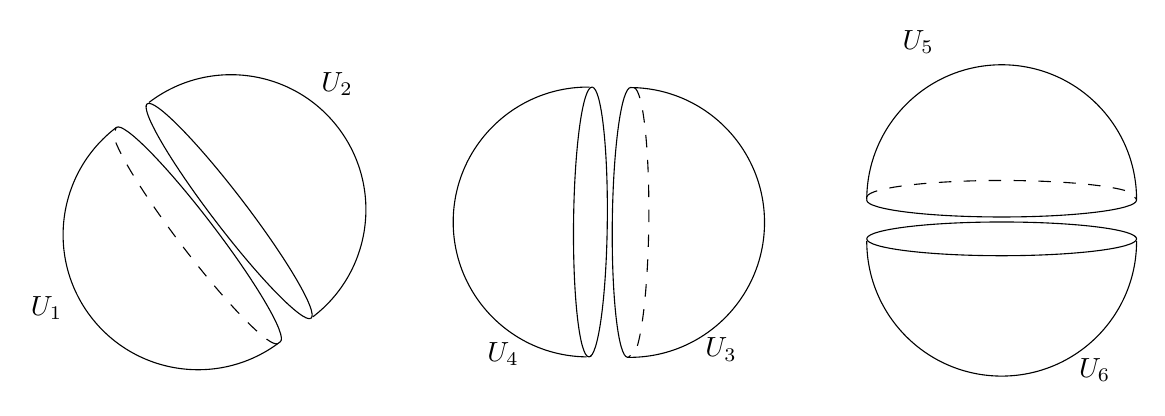
\begin{tikzpicture}[x=0.75pt,y=0.75pt,yscale=-1,xscale=1]
		%uncomment if require: \path (0,300); %set diagram left start at 0, and has height of 300
		
		%Shape: Arc [id:dp8087392079745468] 
		\draw  [draw opacity=0] (610,205) .. controls (610,205) and (610,205) .. (610,205) .. controls (610,240.9) and (580.9,270) .. (545,270) .. controls (509.1,270) and (480,240.9) .. (480,205) -- (545,205) -- cycle ; \draw   (610,205) .. controls (610,205) and (610,205) .. (610,205) .. controls (610,240.9) and (580.9,270) .. (545,270) .. controls (509.1,270) and (480,240.9) .. (480,205) ;  
		%Shape: Arc [id:dp7144643582066421] 
		\draw  [draw opacity=0] (480.02,203.67) .. controls (480.89,199.28) and (509.65,195.75) .. (545,195.75) .. controls (578.58,195.75) and (606.22,198.93) .. (609.64,203.02) -- (545,203.88) -- cycle ; \draw   (480.02,203.67) .. controls (480.89,199.28) and (509.65,195.75) .. (545,195.75) .. controls (578.58,195.75) and (606.22,198.93) .. (609.64,203.02) ;  
		%Shape: Arc [id:dp9774877190814104] 
		\draw  [draw opacity=0] (480,185) .. controls (480,185) and (480,185) .. (480,185) .. controls (480,149.1) and (509.1,120) .. (545,120) .. controls (580.9,120) and (610,149.1) .. (610,185) -- (545,185) -- cycle ; \draw   (480,185) .. controls (480,185) and (480,185) .. (480,185) .. controls (480,149.1) and (509.1,120) .. (545,120) .. controls (580.9,120) and (610,149.1) .. (610,185) ;  
		%Shape: Arc [id:dp7118645098131682] 
		\draw  [draw opacity=0] (609.09,202.51) .. controls (609.69,202.95) and (610,203.41) .. (610,203.88) .. controls (610,208.36) and (580.9,212) .. (545,212) .. controls (509.1,212) and (480,208.36) .. (480,203.88) .. controls (480,203.8) and (480.01,203.73) .. (480.02,203.66) -- (545,203.88) -- cycle ; \draw   (609.09,202.51) .. controls (609.69,202.95) and (610,203.41) .. (610,203.88) .. controls (610,208.36) and (580.9,212) .. (545,212) .. controls (509.1,212) and (480,208.36) .. (480,203.88) .. controls (480,203.8) and (480.01,203.73) .. (480.02,203.66) ;  
		%Shape: Arc [id:dp7962209595423704] 
		\draw  [draw opacity=0] (609.06,183.85) .. controls (609.66,184.29) and (609.98,184.75) .. (609.98,185.22) .. controls (609.98,189.7) and (580.88,193.34) .. (544.98,193.34) .. controls (509.08,193.34) and (479.98,189.7) .. (479.98,185.22) .. controls (479.98,185.14) and (479.99,185.07) .. (480,185) -- (544.98,185.22) -- cycle ; \draw   (609.06,183.85) .. controls (609.66,184.29) and (609.98,184.75) .. (609.98,185.22) .. controls (609.98,189.7) and (580.88,193.34) .. (544.98,193.34) .. controls (509.08,193.34) and (479.98,189.7) .. (479.98,185.22) .. controls (479.98,185.14) and (479.99,185.07) .. (480,185) ;  
		%Shape: Arc [id:dp26854896682720364] 
		\draw  [draw opacity=0][dash pattern={on 4.5pt off 4.5pt}] (480.02,183.67) .. controls (480.89,179.28) and (509.65,175.75) .. (545,175.75) .. controls (578.58,175.75) and (606.22,178.93) .. (609.64,183.02) -- (545,183.88) -- cycle ; \draw  [dash pattern={on 4.5pt off 4.5pt}] (480.02,183.67) .. controls (480.89,179.28) and (509.65,175.75) .. (545,175.75) .. controls (578.58,175.75) and (606.22,178.93) .. (609.64,183.02) ;  
		%Shape: Arc [id:dp8593027572319052] 
		\draw  [draw opacity=0] (345,260.74) .. controls (345,260.74) and (345,260.74) .. (345,260.74) .. controls (345,260.74) and (345,260.74) .. (345,260.74) .. controls (309.1,260.33) and (280.34,230.89) .. (280.75,195) .. controls (281.16,159.1) and (310.6,130.34) .. (346.49,130.75) -- (345.74,195.74) -- cycle ; \draw   (345,260.74) .. controls (345,260.74) and (345,260.74) .. (345,260.74) .. controls (345,260.74) and (345,260.74) .. (345,260.74) .. controls (309.1,260.33) and (280.34,230.89) .. (280.75,195) .. controls (281.16,159.1) and (310.6,130.34) .. (346.49,130.75) ;  
		%Shape: Arc [id:dp5017110012711772] 
		\draw  [draw opacity=0] (347.82,130.78) .. controls (352.2,131.7) and (355.4,160.5) .. (354.99,195.85) .. controls (354.61,229.43) and (351.11,257.03) .. (346.98,260.41) -- (346.87,195.76) -- cycle ; \draw   (347.82,130.78) .. controls (352.2,131.7) and (355.4,160.5) .. (354.99,195.85) .. controls (354.61,229.43) and (351.11,257.03) .. (346.98,260.41) ;  
		%Shape: Arc [id:dp34022749055732393] 
		\draw  [draw opacity=0] (366.49,130.98) .. controls (366.49,130.98) and (366.49,130.98) .. (366.49,130.98) .. controls (402.39,131.39) and (431.15,160.83) .. (430.74,196.72) .. controls (430.33,232.62) and (400.89,261.38) .. (364.99,260.97) -- (365.74,195.97) -- cycle ; \draw   (366.49,130.98) .. controls (366.49,130.98) and (366.49,130.98) .. (366.49,130.98) .. controls (402.39,131.39) and (431.15,160.83) .. (430.74,196.72) .. controls (430.33,232.62) and (400.89,261.38) .. (364.99,260.97) ;  
		%Shape: Arc [id:dp9156415467589833] 
		\draw  [draw opacity=0] (347.5,259.86) .. controls (347.05,260.45) and (346.59,260.76) .. (346.12,260.75) .. controls (341.63,260.7) and (338.33,231.56) .. (338.74,195.66) .. controls (339.16,159.77) and (343.13,130.71) .. (347.62,130.76) .. controls (347.69,130.76) and (347.76,130.77) .. (347.83,130.79) -- (346.87,195.76) -- cycle ; \draw   (347.5,259.86) .. controls (347.05,260.45) and (346.59,260.76) .. (346.12,260.75) .. controls (341.63,260.7) and (338.33,231.56) .. (338.74,195.66) .. controls (339.16,159.77) and (343.13,130.71) .. (347.62,130.76) .. controls (347.69,130.76) and (347.76,130.77) .. (347.83,130.79) ;  
		%Shape: Arc [id:dp7534866185784517] 
		\draw  [draw opacity=0] (366.15,260.05) .. controls (365.7,260.64) and (365.24,260.95) .. (364.78,260.95) .. controls (360.29,260.89) and (356.99,231.75) .. (357.4,195.86) .. controls (357.82,159.96) and (361.79,130.9) .. (366.28,130.95) .. controls (366.35,130.96) and (366.42,130.96) .. (366.49,130.98) -- (365.53,195.95) -- cycle ; \draw   (366.15,260.05) .. controls (365.7,260.64) and (365.24,260.95) .. (364.78,260.95) .. controls (360.29,260.89) and (356.99,231.75) .. (357.4,195.86) .. controls (357.82,159.96) and (361.79,130.9) .. (366.28,130.95) .. controls (366.35,130.96) and (366.42,130.96) .. (366.49,130.98) ;  
		%Shape: Arc [id:dp7058755896129407] 
		\draw  [draw opacity=0][dash pattern={on 4.5pt off 4.5pt}] (367.82,131.01) .. controls (372.2,131.93) and (375.4,160.73) .. (374.99,196.08) .. controls (374.61,229.66) and (371.1,257.26) .. (366.98,260.64) -- (366.87,195.99) -- cycle ; \draw  [dash pattern={on 4.5pt off 4.5pt}] (367.82,131.01) .. controls (372.2,131.93) and (375.4,160.73) .. (374.99,196.08) .. controls (374.61,229.66) and (371.1,257.26) .. (366.98,260.64) ;  
		%Shape: Arc [id:dp6580687340920708] 
		\draw  [draw opacity=0] (134.21,138.15) .. controls (134.21,138.15) and (134.21,138.15) .. (134.21,138.15) .. controls (134.21,138.15) and (134.21,138.15) .. (134.21,138.15) .. controls (162.73,116.35) and (203.52,121.79) .. (225.32,150.31) .. controls (247.13,178.82) and (241.69,219.62) .. (213.17,241.42) -- (173.69,189.79) -- cycle ; \draw   (134.21,138.15) .. controls (134.21,138.15) and (134.21,138.15) .. (134.21,138.15) .. controls (134.21,138.15) and (134.21,138.15) .. (134.21,138.15) .. controls (162.73,116.35) and (203.52,121.79) .. (225.32,150.31) .. controls (247.13,178.82) and (241.69,219.62) .. (213.17,241.42) ;  
		%Shape: Arc [id:dp04807301977746614] 
		\draw  [draw opacity=0] (212.1,242.21) .. controls (208.08,244.19) and (187.81,223.49) .. (166.34,195.4) .. controls (145.94,168.73) and (131.69,144.84) .. (132.85,139.64) -- (172.79,190.47) -- cycle ; \draw   (212.1,242.21) .. controls (208.08,244.19) and (187.81,223.49) .. (166.34,195.4) .. controls (145.94,168.73) and (131.69,144.84) .. (132.85,139.64) ;  
		%Shape: Arc [id:dp5373023961242778] 
		\draw  [draw opacity=0] (197.28,253.57) .. controls (197.28,253.57) and (197.28,253.57) .. (197.28,253.57) .. controls (197.28,253.57) and (197.28,253.57) .. (197.28,253.57) .. controls (168.76,275.37) and (127.97,269.93) .. (106.16,241.41) .. controls (84.36,212.89) and (89.8,172.1) .. (118.32,150.3) -- (157.8,201.93) -- cycle ; \draw   (197.28,253.57) .. controls (197.28,253.57) and (197.28,253.57) .. (197.28,253.57) .. controls (197.28,253.57) and (197.28,253.57) .. (197.28,253.57) .. controls (168.76,275.37) and (127.97,269.93) .. (106.16,241.41) .. controls (84.36,212.89) and (89.8,172.1) .. (118.32,150.3) ;  
		%Shape: Arc [id:dp6075301311311689] 
		\draw  [draw opacity=0] (132.79,140.39) .. controls (132.77,139.64) and (132.95,139.11) .. (133.31,138.83) .. controls (136.88,136.11) and (157.44,157.02) .. (179.25,185.53) .. controls (201.05,214.05) and (215.84,239.38) .. (212.27,242.11) .. controls (212.22,242.15) and (212.15,242.19) .. (212.09,242.22) -- (172.79,190.47) -- cycle ; \draw   (132.79,140.39) .. controls (132.77,139.64) and (132.95,139.11) .. (133.31,138.83) .. controls (136.88,136.11) and (157.44,157.02) .. (179.25,185.53) .. controls (201.05,214.05) and (215.84,239.38) .. (212.27,242.11) .. controls (212.22,242.15) and (212.15,242.19) .. (212.09,242.22) ;  
		%Shape: Arc [id:dp4893987696896971] 
		\draw  [draw opacity=0] (117.98,151.74) .. controls (117.96,150.99) and (118.14,150.47) .. (118.5,150.18) .. controls (122.07,147.46) and (142.64,168.37) .. (164.44,196.89) .. controls (186.24,225.4) and (201.03,250.73) .. (197.46,253.46) .. controls (197.41,253.5) and (197.34,253.54) .. (197.28,253.57) -- (157.98,201.82) -- cycle ; \draw   (117.98,151.74) .. controls (117.96,150.99) and (118.14,150.47) .. (118.5,150.18) .. controls (122.07,147.46) and (142.64,168.37) .. (164.44,196.89) .. controls (186.24,225.4) and (201.03,250.73) .. (197.46,253.46) .. controls (197.41,253.5) and (197.34,253.54) .. (197.28,253.57) ;  
		%Shape: Arc [id:dp5010740042347757] 
		\draw  [draw opacity=0][dash pattern={on 4.5pt off 4.5pt}] (196.21,254.36) .. controls (192.19,256.34) and (171.92,235.64) .. (150.45,207.55) .. controls (130.05,180.87) and (115.8,156.99) .. (116.96,151.78) -- (156.91,202.62) -- cycle ; \draw  [dash pattern={on 4.5pt off 4.5pt}] (196.21,254.36) .. controls (192.19,256.34) and (171.92,235.64) .. (150.45,207.55) .. controls (130.05,180.87) and (115.8,156.99) .. (116.96,151.78) ;  
		
		% Text Node
		\draw (76,230.4) node [anchor=north west][inner sep=0.75pt]    {$U_{1}$};
		% Text Node
		\draw (216,122.4) node [anchor=north west][inner sep=0.75pt]    {$U_{2}$};
		% Text Node
		\draw (401,250.4) node [anchor=north west][inner sep=0.75pt]    {$U_{3}$};
		% Text Node
		\draw (296,252.4) node [anchor=north west][inner sep=0.75pt]    {$U_{4}$};
		% Text Node
		\draw (496,102.4) node [anchor=north west][inner sep=0.75pt]    {$U_{5}$};
		% Text Node
		\draw (581,260.4) node [anchor=north west][inner sep=0.75pt]    {$U_{6}$};
		
		
	\end{tikzpicture}
\end{figure}
\end{problem}
\begin{solution}
	For the set $ U_1 \cap U_4 $ we have
	\[ U_1 \cap U_4 = \set{(x,y,z) \in S^2\ :\ x>0 \text{ and } y < 0 }. \]
	Thus we will have
	\[ \phi_4(U_1\cap U_4) = \set{(x,z)\in \R^2 \ :\ x^2 + z^2 \leq 1,\ x>0}. \]
	Thus we can write
	\[ (\phi_1 \circ \inv{\phi_4})(\langle x,z \rangle ) = \phi_1(\langle x,-\sqrt{1-(x^2+y^2)},z \rangle) = \langle -\sqrt{1-(x^2+y^2)},z \rangle  \]
	This is indeed a $ C^\infty $ vector valued function, since each component is a $ C^\infty $ function. Now to evaluate $ \phi_4 \circ \inv{\phi_1}: \phi_1(U_1 \cap U_4) \to \phi_4(U_1\cap U_4) $ we need to first evaluate the set $ \phi_1(U_1 \cap U_4) $. For this set we have
	\[ \phi_1(U_1 \cap U_4) = \set{(z,y)\in\R^2\ :\ z^2 + y^2 \leq 1, y < 0}. \]
	Then we can write
	\[ (\phi_4 \circ \inv{\phi_1})(\langle y,z \rangle ) = \phi_4(\langle \sqrt{1-(y^2+z^2)}, y,z  \rangle) = \langle \sqrt{1-(y^2+z^2)} , z \rangle. \]
	This is indeed a $ C^\infty $ vector valued function. 
	
	To evaluate the function $ \phi_6 \circ \inv{\phi}_1: \phi_1(U_1 \cap U_6) \to \phi_6(U_1 \cap U_6) $, we first need to determine the domain of this function. First observe that 
	\[ U_1 \cap U_6 =  \set{(x,y,z) \in S^2\ :\ x>0 \text{ and } y<0}, \]
	which is the same as $ U_1 \cap U_4 $. Then for the domain of the function of interest we can write
	\[ \phi_1(U_1 \cap U_6) = \set{(y,z) \in \R^2 :\ z^2 + y^2 \leq 1 \text{ and } y<0}, \]
	\[ (\phi_6 \circ \inv{\phi_1})(\langle y,z \rangle) = \phi_6(\langle \sqrt{1-(y^2+z^2)},y,z \rangle) = \langle \sqrt{1-(y^2+z^2)}, y \rangle. \]
\end{solution}

\begin{problem}[Existence of a coordinate neighborhood (from W. Tu)]
	Let $ \set{(U_\alpha, \phi_\alpha)}_{\alpha \in I} $ be the maximal atlas on manifold $ M $. For any open set $ U $ in $ M $ and a point $ p \in U $, prove the existence of a coordinate open set $ U_\alpha $ such that $ p \in U_\alpha \subset U $.
\end{problem}
\begin{solution}
	Since $ \set{(U_\alpha,\phi_\alpha)}_{\alpha \in I} $ is an atlas, then for $ p \in U $ given as above, we can find some $ \alpha_1 \in I $ such that $ p \in U_{\alpha_1} $. Consider the open set $ W = U_{\alpha_1} \cap U $. The chart $ (W, \phi_{\alpha_1}|_W) $ is in the atlas (since it is maximal), i.e. $ \exists \alpha \in I $ such that $ (U_\alpha, \phi_\alpha) = (W, \phi_{\alpha_1}|_W) $. This completes the proof.
\end{solution}

\begin{problem}[An atlas for a product manifold (from W. Tu)]
	Prove the following proposition.
	\begin{proposition}
		If $ \set{(U_\alpha,\phi_\alpha)} $ and $ \set{(V_i,\psi_i)} $ are $ C^\infty $ atlases for the manifold $ M $ and $ N $ of dimensions $ m $ and $ n $, respectively, then the collection 
		\[ \set{(U_\alpha \times V_i,\phi_\alpha \times \psi_i)} \] where
		\[ \phi_\alpha \times \psi_i\ :\ U_\alpha \times V_i \to \R^m \times \R^n \]
		of charts is a $ C^\infty $ atlas on $ M\times N $. Therefore, $ M\times N $ is a $ C^\infty $ manifold of dimension $ m+n $.
	\end{proposition}
\end{problem}
\begin{solution}
	In order to show that the collection $ \frak{U} = \set{(U_\alpha \times V_i, \phi_\alpha \times \psi_i)} $ is an atlas for $ M\times N $, we need to show that charts are pairwise compatible as well as the set covering the whole space. To show that the chart covers the whole space $ M\times N $, let $ (p_1,p_2) \in M\times N $. Then $ p_1 \in M $ and $ p_2 \in N $. Then there are two coordinate open sets such that $ p_1 \in U_{\alpha_1} $ and $ p_2 \in V_{i_1} $. Thus the coordinate open set $ U_{\alpha_1} \times V_{i_1} $ contains the point $ (p_1,p_2) $.
	
	To show that two any two charts in the collection $ \frak{U} $ are compatible, let $ (U_{\alpha_1} \times V_{i_1},\phi_{\alpha_1}\times \psi_{i_1}) $ and $  (U_{\alpha_2} \times V_{i_2},\phi_{\alpha_2}\times \psi_{i_2}) $ be two  charts. We claim that the corresponding coordinate maps are $ C^\infty $. This follows directly from the fact the each component of the map these coordinate maps are $ C^\infty $.
\end{solution}


\chapter{Tangent Spaces}

\section{Tangent Spaces}

For several reasons, the notion of tangent space is more easily developed using algebraic view point rather than the geometric one. Then we can easily construct our geometric intuition from using the developed theory. We start with the notion of derivation.


\begin{definition}[Derivation at a point]
	Let $ M $ be a manifold and $ p $ a point of manifold. Let $ C_p^\infty(M) $ denote the germ of $ C^\infty $ functions at $ p $. Derivation at $ p $ is a linear map 
	\[ D: C_p^\infty(M) \to \R \]
	such that for $ f,g \in C_p^\infty(M) $ we have
	\[ D(fg) = D(f)g + fD(g). \]
\end{definition}
The definition above is a purely algebraic one.
\begin{remark}
	The set of all point derivations at $ p $ forms a vector space.
\end{remark}

\begin{definition}[Tangent space]
	Let $ M $ be a manifold and $ p \in M $. The tangent space at $ p $ denoted by $ T_p(M) $ is the vector space of all point derivations at $ p $.
\end{definition}
In the following proposition we will see a very familiar point derivation.
\begin{proposition}[Partial derivative $ \partial/\partial x^i |_p $ is a tangent vector]
	Let $ M $ be a manifold and $ p \in M $. Let $ (U,\phi) $ be a coordinate chart containing $ p $ and $ f:M \to \R $ a function defined at a neighborhood of $ p $. By definition we have
	\[ \frac{\partial }{\partial x^i}\big|_p f = \frac{\partial}{\partial r^i}\big|_{\phi(p)} (f\circ\inv{\phi}) \]
	where $ x^i = r^i \circ f $ with $ r^i $ as the standard coordinate function of $ \R^n $. The map $ \frac{\partial}{\partial x^i}\big|_{p} $ is a point derivation at $ p $, thus a tangent vector.
\end{proposition}
\begin{proof}
	First observe that $ \partial/\partial x_i|_p $ is indeed a linear map from $ C_p^\infty(M) $ to $ \R $. Let $ f,g \in C_p^\infty(U) $ and $ (U,x^1,\cdots,x^n) $ a coordinate chart. Then we have
	\begin{align*}
		\frac{\partial}{\partial x^i}\big|_p (fg) &=  \frac{\partial}{\partial  r^i}\big|_{\phi(p)}((fg)\circ \inv{\phi} ) = \frac{\partial}{\partial  r^i}\big|_{\phi(p)}(f\circ\inv{\phi} \cdot g\circ\inv{\phi}) \\
		&= \frac{\partial}{\partial  r^i}\big|_{\phi(p)}(f\circ\inv{\phi})\cdot g(p) + f(p)\cdot \frac{\partial}{\partial  r^i}\big|_{\phi(p)} (g\circ\inv{\phi})\\
		&=(\frac{\partial}{\partial  x^i}\big|_{p}f ) g + f(\frac{\partial}{\partial  x^i}\big|_{p} g).
	\end{align*}
\end{proof}

\begin{definition}[Differential of a smooth map]
	Let $ F:N\to M $ be a smooth map between manifolds. This map induces a \emph{linear} map  called the \emph{differential of $ F $}
	\[ F_*: T_p N \to T_{F(p)}M \]
	where for $ X_P \in T_p N $ we have
	\[ (F_*(X_p))f = X_p(f\circ F) \]
	where $ f $ is a germ at $ p $.
\end{definition}

\begin{proposition}
	Let $ F:N\to M $. It differential $ F_* $ is a derivation at $ F(p) $ for $ p \in N $. 
\end{proposition}
\begin{proof}
	See \autoref{prob:DifferentialOfAMapIsADerivation}
\end{proof}

\subsubsection{Differential of a map between Euclidean spaces}
To see what kind of an object is the differential of a map, we calculate it explicitly on Euclidean spaces. Let $ F:\R^n \to \R^m $ be a map and let $ x^1,\cdots,x^n $ be the standard coordinate functions of $ \R^n $ while $ y^1,\cdots,y^m $ be the standard coordinate functions of $ \R^m $. Let $ p \in \R^n $. since $ F_* $ is a linear map between two vector spaces, then we can write it as a matrix once we fix the basis for the spaces. The basis for $ T_p(\R^n) $ is the set $ \set{\partial/\partial x^i|_p}_{i} $, while for $ T_p(\R^m) $ is $ \set{\partial/\partial y^j|_p}_j $. To get the matrix representation of $ F_* $ we need to find its effect on the basis vectors
\[ F_*(\frac{\partial}{\partial  x^j}\big|_{p}) = \sum_{k} a^k_j\  \frac{\partial}{\partial  y^k}\big|_{F(p)}. \]
By applying it on $ y_i $ we will get
\[ a_j^i = F_*(\frac{\partial}{\partial  x^j}\big|_{p})y^i = \frac{\partial}{\partial  x^j}\big|_{p} (y^i \circ F) =  \frac{\partial}{\partial  x^j}\big|_{p}F^i. \]
This is precisely the Jacobian matrix of $ F $ evaluated at $ p $.

\subsubsection{The Chain Rule}
A nice thing behind this algebraic point of view is that we can now write the notion of chain rule in a much simpler form. The following propositions captures this ides.

\begin{proposition}[The chain rule]
	\label{prop:ChainRule}
	Let $ F: N \to M $ and $ G:M\to P $ be maps between manifolds, and $ p \in N $. Then the differential of $ F $ at $ p $ and $ G $ at $ F(p) $ are linear maps
	\[ T_pN \xrightarrow{F_{*,p}} T_pM \xrightarrow{G_{*,F(p)}} T_pP. \]
	Then we have
	\[ (G\circ F)_{*,p} = G_{*,F(p)} F_{*,p}. \]
\end{proposition}
\begin{proof}
	Let $ X_p \in T_p(N) $. From definition we have for some $ f: G \to \R $ we have
	\[ ((G\circ F)_{*,p}X_p)f = X_p(f\circ G\circ F) = X_p ((f\circ G)\circ F) = (F_{*,p}X_p)(f\circ G).\]
	Let $ Y_q = F_{*,p}X_p $ where $ q = F(p) $. Then 
	\[ Y_q (f\circ G) = (G_{*,q}Y_q) f.  \]
	This implies that 
	\[ (G\circ F)_{*,p} = G_{*,q} F_{*,p} \]
	and this completes the proof.
\end{proof}

\begin{example}
	Let $ F:\R \to \R^3 $ and $ G:\R^3 \to \R $. Then the differential of the composite function $ G\circ F $ is the matrix multiplication of the differential of each map. I.e.
	\[ (G \circ F)_* = G_* F_* = (G_x\ G_y\ G_z)\cdot 
	\begin{pmatrix}
		F_1' \\
		F_2' \\
		F_3'
	\end{pmatrix}
	= G_x F_1' + G_y F_2' + G_z F_3' 
	= \frac{\partial G}{\partial x} \frac{d F_1}{dt} 
	+\frac{\partial G}{\partial y} \frac{d F_2}{dt} 
	+\frac{\partial G}{\partial z} \frac{d F_3}{dt},
	 \]
	 which is the same chain rule in calculus.
\end{example}
Writing the chain rule in this form not only is visually appealing, but also we can deduce two important Corollaries from it as follows.

\begin{corollary}[Diffeomorphism of Manifolds vs. Isomorphism of Tangent Spaces]
	Let $ F:N\to M $ be a diffeomorphism of manifolds and $ p \in N $. Its differential $ F_* $ is an isomorphism of tangent spaces $ T_pN $ and $ T_{F(p)}M $.
\end{corollary}
\begin{proof}
	$ F $ being a diffeomorphism of manifolds, it implies that we have $ G: M \to N $ such that $ G\circ F = \mathbbm{1}_N $ and $ F\circ G = \mathbbm{1}_M $. Now using \autoref{prop:ChainRule} we can write
	\begin{align*}
		(G\circ F)_* = G_* \circ F_* = (\mathbbm{1}_N)_* = \mathbbm{1}_{T_pN}\\
		(F\circ G)_* = F_* \circ G_* = (\mathbbm{1}_M)_* = \mathbbm{1}_{T_{F(p)}M}.
	\end{align*}
	This shows that $ F_* $ and $ G_* $ are the right and left inverses of each other, hence an isomorphism of vector spaces.
\end{proof}
\begin{corollary}[Invariance of Dimension]
	Let $ U \subset \R^n $ and $ V \subset R^m $ be open subsets that are diffeomorphic. Then $ m = n $.
\end{corollary}
\begin{proof}
	Let $ F: U \to V $ be a diffeomorphism and $ p \in U $. Then $ F_* $ is an isomorphism of tangent spaces $ T_pU $ and $ T_{F(p)}V $, thus of the same dimension. Since in a Euclidean space the tangent space has the same dimension as the space itself (by definition and the way that we construct a basis for tangent space using the standard coordinate vectors) then this implies that $ n = m $.
\end{proof}

\begin{corollary}[Tangent Space Has the Same Dimension as Manifold]
	\label{cor:TangentSpaceIsoMorphismToRn}
	Let $ M $ be a manifold of dimension $ n $ and $ p \in M $. Then $ T_p(M) $ is isomorphic to $ \R^n $ and has dimension $ n $.
\end{corollary}
\begin{proof}
	Let $ (U,\phi) $ be a coordinate chart containing the point $ p $. Since $ M $ is assumed to be a smooth manifold, then the coordinate map $ \phi $ automatically upgrades to a diffeomorphism between $ U $ and $ \R^n $. Thus the tangent spaces $ T_p(U) $ and $ T_{\phi(p)}(\R^n) $ are isomorphic. This implies that $ T_p(U) $ is also of dimension $ n $.
\end{proof}

\section{Basis for the Tangent Space at a Point}
\begin{proposition}[Differential of a Coordinate Map]
	\label{prop:DifferentialOfACoordinateMap}
	Let $ M $ be a manifold, $ p \in M $, and $ (U,x^1\cdots,x^n) $ a coordinate chart containing $ p $. Then
	\[ \phi_* (\frac{\partial}{\partial  x^i}\big|_{p}) = \frac{\partial}{\partial  r^i}\big|_{\phi(p)} \]
\end{proposition}
\begin{proof}
	This follows immediately from the definition. Namely for a function $ f $ defined on $ U $ we have
	\begin{align*}
		(\phi_*(\frac{\partial}{\partial  x^i}\big|_{p}))f = \frac{\partial}{\partial  x^i}\big|_{p}(f\circ \phi) = \frac{\partial}{\partial  r^i}\big|_{\phi(p)}(f\circ\phi\circ\inv{\phi}) = \frac{\partial}{\partial  r^i}\big|_{\phi(p)}f.
	\end{align*}
	This implies 
	\[ \phi_*(\frac{\partial}{\partial  x^i}\big|_{p}) = \frac{\partial}{\partial  r^i}\big|_{\phi(p)}. \]
\end{proof}
\begin{remark}
	\label{remark:differentialOfCoordinateMapActingOnBases}
	Remember that in \autoref{def:DirectionalDerivativeOnManifold} we defined
	\[ \frac{\partial}{\partial  x^i}\big|_{p} f = \frac{\partial}{\partial  r^i}\big|_{\phi(p)}(f\circ\inv{\phi}).\tag{\eighthnote} \]
	where $ (U,\phi) $ is a coordinate chart containing $ p $ and $ x^i = r^i \circ \phi $. The proposition above justifies this definition. This proposition states that $ T_p(M) \simeq T_{\phi(p)}(R^n) $ with $ \phi_* $ as an isomorphism. This basically means that $ \partial/\partial x^i $ maps to $ \partial/\partial r^i $ with map $ \phi_* $, or equivalently,  $ \partial/\partial r^i $ maps to $ \partial/\partial x^i $ with the map $ \inv{\phi}_* $. I.e.
	\[ \frac{\partial}{\partial  x^i}\big|_{p} \mapsto \frac{\partial}{\partial  r^i}\big|_{\phi(p)} \quad\text{via } \phi_* \]
	and 
	\[ \frac{\partial}{\partial  r^i}\big|_{p} \mapsto \frac{\partial}{\partial  x^i}\big|_{\phi(p)} \quad\text{via } \inv{\phi}_* \]
	Thus starting with the LHS of $ (\eighthnote) $ we can write
	\[ \frac{\partial}{\partial  x^i}\big|_{p}f = (\inv{\phi}_*(\frac{\partial}{\partial  r^i}\big|_{\phi(p)}))f = \frac{\partial}{\partial  r^i}\big|_{\phi(p)}(f\circ \inv{\phi}).  \]
\end{remark}


\begin{proposition}[Basis for Tangent Space]
	\label{prop:BasisForTangetSpace}
	Let $ M $ be a manifold of dimension $ n $ and $ p \in M $. Then the vectors $ \partial/\partial x^1|_p,\cdots, \partial/\partial x^n|_p $ is a basis for the tangent space $ T_p(M) $.
\end{proposition}
\begin{proof}
	Let $ (U,\phi) $ be a coordinate chart containing $ p $. By \autoref{cor:TangentSpaceIsoMorphismToRn} we see that $ T_pM $ is isomorphic to $ \R^m $ with $ \phi_* $ as a possible isomorphism. Since an isomorphism of vector spaces carries basis to a basis, and by \autoref{prop:DifferentialOfACoordinateMap} $ \phi_* $ maps the standard basis $ \frac{\partial}{\partial  r^1}\big|_{\phi(p)},\cdots,\frac{\partial}{\partial  r^n}\big|_{\phi(p)} $ to $ \partial/\partial x^1|_p,\cdots, \partial/\partial x^n|_p $ respectively, then this forms a basis for $ T_p(M) $.
\end{proof}

\begin{remark}
	For a point $ p \in M $, once we fix a coordinate chart containing $ p $ we have a basis for $ T_p(M) $
\end{remark}


\begin{proposition}[Transition Matrix for Coordinate Vectors]
	Let $ M $ be a manifold and $ p \in M $. Let $ (U,\phi=(x^1,\cdots,x^n)) $ and $ (V,\psi=(y^1,\cdots,y^n)) $ be two coordinate charts containing $ p $. By \autoref{prop:BasisForTangetSpace} the following two collection of tangent vectors form two possible bases for $ T_pM $
	\[ \set{ \frac{\partial}{\partial  x^1}\big|_{p}, \cdots, \frac{\partial}{\partial  x^n}\big|_{p} }, \qquad \set{\frac{\partial}{\partial  y^1}\big|_{p},\cdots,\frac{\partial}{\partial  y^n}\big|_{p}}. \]
	The transition rule between these two basis is given by
	\[ \frac{\partial}{\partial  x^j} = \sum_{i} \frac{\partial y^i}{\partial x^j} \frac{\partial}{\partial y^i},  \]
	on $ U \cap V $.
\end{proposition}
\begin{proof}
	We can think of this as $ \psi $ is a map between manifolds, i.e. $ \psi: U\cap V \subset M \to \R^n $. Considering the chart $ (W,\mathbbm{1}_{\R^n}) $ for the target manifold of $ \psi $, what we are looking after is to see how does $ \psi_* $ maps the tangent vector $ \partial/\partial x^j $. For $ \psi_* $ it is a map from $ T_pN $ to $ T_{\psi(p)}\R^n $ where the basis for $ T_{\psi(p)}\R^n $ is the collection $ \set{\partial /\partial r^i}_i $. Thus we can write
	\[ \psi_*(\partial/\partial x^j|_p) = \sum_k a_j^k \partial/\partial r^k|_{\psi(p)}. \]
	Applying $ r^i $ to both sides will result in 
	\[ a_j^i  =  \phi_*(\partial/\partial x^j|_p) r^i = \partial/\partial x^j|_p (r^i\circ\phi) = \partial/\partial x^j|_p y^i. \]
	So far we have shown that 
	\[ \psi_*(\frac{\partial }{\partial x^j}) = \sum_i \frac{\partial y^i}{\partial x^j}\frac{\partial}{\partial r^i} \]
	Now by applying $ \inv{\psi_*} $ to both sides and using the observation in \autoref{remark:differentialOfCoordinateMapActingOnBases} we can write
	\[ \frac{\partial}{\partial x^j} = \sum_i \frac{\partial y^i}{\partial x^j} \frac{\partial}{\partial y^i} \]
	where we have used the fact that $ \inv{\psi}_* $ is linear.
\end{proof}
\begin{remark}
	The relation above can be written symbolically as matrix multiplication
		\[ 
	\begin{bmatrix}
		\partial/\partial x^1 \\
		\partial/\partial x^2 \\
		\vdots \\
		\partial/\partial x^n
	\end{bmatrix} = 
	\begin{pmatrix}
		\partial y^1/\partial x^1 & \partial y^1/\partial x^2 &  \cdots & \partial y^1/\partial x^n \\
		\partial y^2/\partial x^1 & \partial y^2/\partial x^2 &  \cdots & \partial y^2/\partial x^n \\
		\vdots & \vdots & \ddots & \vdots \\
		\partial y^n/\partial x^1 & \partial y^n/\partial x^2 &  \cdots & \partial y^n/\partial x^n
	\end{pmatrix}^T
	\begin{bmatrix}
		\partial/\partial y^1 \\
		\partial/\partial y^2 \\
		\vdots \\
		\partial/\partial y^n
	\end{bmatrix}
	\]
\end{remark}


\subsubsection{A Local Expression for the Differential}
We start with the following proposition.
\begin{proposition}[Local Expression for the Differential]
	Let $ F: N\to M $ be a map between manifolds, and $ p \in N $. Let $ (U,x^1\cdots,x^n) $ be a coordinate chart in $ N $ containing $ p $ and $ (V,y^1,\cdots,y^n) $ containing $ F(p) $ be a coordinate chart in $ M $. Relative to the bases $ \set{\partial /\partial x^j|_{p}} $ for $ T_pN $ and $ \set{\partial/\partial y^i|_{F(p)}} $ for $ T_pM $, the differential $ F_*: T_pN \to T_pM $ is represented by the matrix
	\[ [\partial F^i/\partial x^j(p)], \]
	where $ F^i = y^i \circ F $.
\end{proposition}
\begin{remark}
	We can state the inverse function theorem for manifolds \autoref{thm:InverseFunctionTheoremForManifolds} in a coordinate free description: A $ C^\infty $ function $ F:N\to M $ is locally invertible at point $ p\in N $ if and only if $ F_*: T_pN \to T_pM $ is an isomorphism of vector spaces.
\end{remark}


\section{Curves in a Manifold}
The notion of a curve in a manifold is a very important one as it will allow us to define the tangent space in an alternative way. We start by the definition of a curve in a manifold.

\begin{definition}[Curves in a Manifold]
	Let $ M $ be a manifolds and $ p \in M $. a \emph{curve} in manifold is a map
	\[ c: (a,b) \to M. \]
	Usually $ 0 \in (a,b) $ and we say $ c $ is a \emph{curve starting at $ p $} if $ c(0) = p $. The \emph{velocity vector} $ c'(t_0) $ of the curve at time $ t_0 \in (a,b) $ is defined to be
	\[ c'(t_0) = c_*(\frac{d}{dt}\big|_{t_0}) \in T_{c(t_0)}M. \]
\end{definition}

\begin{remark}
	Note that the velocity vector of the curve $ c $ at time $ t_0 $ denoted by $ c'(t_0) $ is a tangent vector at $ T_{c(p)}M $. This in particular can be a source of confusion when the target space of the curve is $ \R $. That is because in the calculus the notation $ c'(t) $ is the derivative of a real-valued function and is therefore a scalar. If it is necessary to distinguish between these two meanings of $ c'(t) $ when $ c $ maps into $ \R $, we will write $ \dot{c}(t) $ for the calculus derivative. For a clarification on this point visit \autoref{prob:VelocutyVecotrAndCalculusNotation}.
\end{remark}
\begin{remark}
	Alternative notations for $ c'(t_0) $ are
	\[ \frac{d}{dt}\big|_{t_0} c, \qquad \frac{dc}{dt}(t_0). \]
	However, I prefer the notation introduced in the definition box above as it has more emphasis on the fact that $ c'(t) $ is a vector in $ T_pM $.
\end{remark}

\begin{example}{Velocity vector of a curve is consistent with the results in calculus}
	\label{example:VelocityVectorWorkedExample}
	In this example we will demonstrate that the notion of the velocity vector of a curve is consistent with the similar notion in calculus. Define $ c:\R \to \R^2 $. 
	\[ c(t)  = (t^2, t^3). \]
	The velocity vector $ c'(t) $ is in tangent space $ T_{c(t)}\R^2 $. Let $ (\R^2, \mathbbm{1}_{\R^2}) $ be the atlas for manifold $ \R^2 $. Then we can write $ c'(t)$ in terms of the basis for tangent space.
	\[ c'(t) = a \frac{\partial}{\partial  x}\big|_{c(t)} + b \frac{\partial}{\partial  y}\big|_{c(t)}. \] 
	To determine the coefficients we apply the standard coordinate function $ x,y $ to both sides and we will get
	\[ c'(t)x = a, \qquad c'(t)y = b. \]
	From definition we have
	\[ c'(t) x = c_*(\frac{d}{dt}\big|_t) x = \frac{d}{dt}\big|_t (x\circ c) = \frac{d}{dt}\big|_t (t^2) = 2t.   \]
	Similarly we can get $ c'(t) y = 3t^2$. Thus
	\[ c'(t) = (2t) \frac{\partial}{\partial  x}\big|_{c(t)} + (3t^2) \frac{\partial}{\partial  y}\big|_{c(t)}. \]
\end{example}

The steps that we took in the example above motivates us for the following proposition.
\begin{proposition}[Velocity Vector in a Local Coordinate]
	\label{prop:VelocityVectorInLocalCorodinate}
	Let $ c:(a,b)\to M $ be a smooth curve, and let $ (U,x^1,\cdots,x^n) $ be a coordinate chart about $ c(t) $. Write $ c^i = x^i\circ c $ for the i-th component of $ c $ in the chart. Then $ c'(t) \in T_{c(t)}M $ is given by
	\[ c'(t) = \sum_i \dot{c}_i \frac{\partial}{\partial x^i}\big|_{c(t)}. \] 
	Thus relative to the bases $ \set{\partial /\partial x^i|_p} $ for $ T_{c(t)}M $ the velocity vector $ c'(t) $ can be written as
	\[ \begin{bmatrix}
		\dot{c}_1(t) \\
		\dot{c}_2(t) \\
		\vdots \\
		\dot{c}_n(t)
	\end{bmatrix} \]
\end{proposition}
\begin{proof}
	First, observe that by definition $ c'(t) \in T_{c(t)}M  $ thus can be written in the local coordinate  of $ T_{c(t)}M $ as
	\[ c'(t) = \sum_i a^i \frac{\partial}{\partial x^i}\big|_{c(t)}. \]
	Now we apply both sides to $ x_j $, and simply use the definition of the differential of a map and write
	\[x^j = c_*(\frac{d}{dt}\big|_{t}) x^j  =  \frac{d}{dt}\big|_{t}(x^j\circ c) = \dot{c}^j(t). \]
	This completes the proof.
\end{proof}

So far, we observed that every smooth curve $ c $ at $ p $ in a manifold $ M $ gives rise to a tangent vector in $ T_pM $. The following proposition states the converse of this, i.e. for every tangent vector in tangent space $ T_pM $ there exists a curve passing through $ p $.

\begin{proposition}[Existence of a Curve with a Given Initial Vector]
	For any point $ p $ in a manifold $ M $ and any tangent vector $ X_p \in T_pM $, there are $ \epsilon>0 $ and a smooth curve $ c:(-\epsilon,\epsilon) \to M $ such that $ c(0) = p $ and $ c'(0) = X_p $
\end{proposition}
\begin{proof}
	Let $ p \in M $ and $ X_p \in T_pM $.  Let $ (U,\phi = (x^1,\cdots,x^n)) $ be a coordinate chart centered at $ p $. The differential of $ \phi $ given by $ \phi_* $ maps $ X_p $ to $ Y_{\mathbf{0}} \in T_\mathbf{0}\R^n $. For instance, assume 
	\[ X_p = \sum_i a^i \frac{\partial}{\partial  x^i}\big|_{p}. \]
	Applying $ \phi_* $ to both sides and using \autoref{prop:DifferentialOfACoordinateMap} we will get
	\[ Y_\mathbf{0} =  \sum_i a^i \frac{\partial}{\partial  r^i}\big|_{\mathbf{0}}  \]
	where $ r^i $ is the standard coordinate function of $ \R^n $. Define the smooth curve $ \gamma: (-\epsilon, \epsilon) \to \R^n $ given by
	\[ \gamma(t) = (a^1t, \cdots, a^n t). \]
	For small enough $ \epsilon $ this curve is in $ \phi(U) $. We claim that the curve $ c:(-\epsilon,\epsilon)\to M $ given by
	\[ c = \inv{\phi} \circ \gamma \] 
	has the desired property. First, observe by definition we will have $ c(0) = p $
	\[ c(0) = \inv{\phi}(\gamma(0)) = p. \]
	For $ c'(0) $ we use the definition
	\[ c'(0) = c_*(d/dt|_{0}) = (\inv{\phi}\circ \gamma)_*(d/dt|_{0}) = (\inv{\phi}_*  \gamma_*)(d/dt|_{0})  \]
	It now remains to calculate the $ (\inv{\phi}_* \gamma_*) $. To calculate this, first observe that $ \gamma_* $ maps $ d/dt|_0 $ to $ Y_\mathbf{0} $. And also observe that $ \inv{\phi}_* $ maps $ X_p $ to $ Y_\mathbf{0} $. I.e.
	\[ Y_\mathbf{0} = \phi_* X_p, \qquad Y_\mathbf{0} = \gamma_* \frac{d}{dt}\big|_0. \]
	Then we will get
	\[ \phi_* X_p = \gamma_* \frac{d}{d  t}\big|_{0} \implies X_p = \inv{\phi}_* \gamma_* \frac{d}{dt}\big|_0. \]
	Thus we have
	\[ c'(0) =  \inv{\phi}_* \gamma_* \frac{d}{dt}\big|_0. = X_p\]
	and this completes the proof.
\end{proof}

Now using the notion of curves, we can calculate the differential of a map between manifolds via curves. The following proposition discusses this statement.
\begin{proposition}[Computing Differentials Using Curves]
	\label{prop:curvesToComputeDifferential}
	Let $ F: N  \to M$ be a smooth map between manifolds, and $ p \in N $ and $ X_p \in T_pN $. Let $ c $ be a curve on $ N $ such that $ c(0) = p $, and $ c'(0) = X_p $. Then
	\[ F_{*,p} X_p = (F\circ c)' (0). \]
\end{proposition}
\begin{proof}
	We simply follow the definition
	\[(F\circ c)'(0) = (F\circ c)_* (\frac{d}{dt}\big|_0) = F_* c_* (\frac{d}{dt}\big|_0) = F_* \left(  c_* (\frac{d}{dt}\big|_0) \right) = F_* X_p \]
	and this completes the proof.
\end{proof}


\section{Immersion and Submersion}
We start with the definitions of Immersion and Submersion.
\begin{definition}[Immersion and Submersion]
	Let $ F:N\to M $ be a smooth map, and let $ F_{*,p} $ denote its differential at a point $ p \in N $. Then 
	\begin{itemize}[noitemsep]
		\item $ F $ is an Immersion if and only if $ F_{*,p} $ is injective.
		\item $ F $ is a Submersion if and only if $ F_{*,p} $ is surjective.
	\end{itemize}
\end{definition}

Now we can define the notion of critical point and regular points of a mapping.
\begin{definition}[Critical and Regular points of a smooth map between manifolds]
	Let $ F:N \to M $ be a smooth map between manifolds. A point point $ p  \in N$ is
	\begin{itemize}[noitemsep]
		\item a \emph{critical point} if $ F_{*,p} $ fails to be surjective, and
		\item a \emph{regular point} if $ F_{*,p} $ is surjective.
	\end{itemize}
	A point $ q \in M $ is critical value of the map $ F $ if it is the image of a critical point.
\end{definition}

The following proposition gives a more intuitive characterization of the critical points of function defined from a manifold to the real number line.

\begin{proposition}[Critical points of a map to real number line]
	Let $ f: N \to \R $ be a smooth map from manifold $ N $ to the real number line. A point $ p \in N $ is a critical point of the map $ f $ in and only if all of its partial derivatives relative to some chart $ (U,\phi=(x^1,\cdots,x^n)) $ are zero at $ p $, i.e.
	\[ \frac{\partial }{\partial x^i}\big|_{p} f = 0 \qquad \text{for all } i = 1,\cdots, n. \]
\end{proposition}
\begin{proof}
	The differential of $ f $ in the local coordinates can be written as the matrix
	\[ f_{*,p} = [ \frac{\partial}{\partial  x^1}\big|_{p} f, \cdots, \frac{\partial}{\partial  x^n}\big|_{p} f ]. \]
	The point $ p $ is a critical point if and only if $ f_{*,p} $ is not surjective. Since the image of $ f_{*,p} $ is $ \R $, then its column space is either one dimensional or zero dimensional. Thus $ f_{*,p} $ is not surjective if and only if all of its entries are zero, i.e.
	\[ \frac{\partial }{\partial x^i}\big|_{p} f = 0 \qquad \text{for all } i = 1,\cdots, n. \]
\end{proof}


\newpage




\section{Summary}
\begin{summary}[Coordinate Map and Its Differential]
	Let $ M $ be a manifold and $ p \in M $. Let $ (U,\phi) $ be a coordinate chart containing $ p $. We saw in \autoref{propositio:coordinateMapsAreSmooth} that $ \phi $ is a diffeomorphism between $ U $ and $ \R^n $. In \autoref{cor:TangentSpaceIsoMorphismToRn} we also saw that $ T_p(U) $ is isomorphic to $ T_{\phi(p)}(\R^n) $. In a nutshell
	\begin{quote}
		Under a coordinate chart $ (U,\phi) $, $ U $ is diffeomorphic to $ \R^n $ and at a point $ p \in U $ the tangent space at $ p $, i.e. $ T_p(U) $, is isomorphic to the tangent space at $ \phi(p) $, i.e. $ T_\phi(p)_n $.
	\end{quote}
\end{summary}

\begin{summary}[Differential of a Map Between Euclidean Spaces]
	Let $ F: \R^n \to \R^m $. It differential at point $ p \in \R^n $ is its Jacobian matrix evaluated at point $ p $.
	\[ F_* = 
	\begin{pmatrix}
		\frac{\partial F^1}{\partial x^1} & \cdots & \frac{\partial F^1}{\partial x^n} \\
		\frac{\partial F^2}{\partial x^1} & \cdots & \frac{\partial F^2}{\partial x^n} \\
		\vdots & \ddots & \vdots \\
		\frac{\partial F^m}{\partial x^1} & \cdots & \frac{\partial F^m}{\partial x^n}
	\end{pmatrix}(p)
	 \]
\end{summary}

\begin{summary}{Differential of a coordinate map acting on a tangent vector}
	Let $ M $ be a manifold and $ (U,\phi = (x^1,\cdots,x^n)) $ a coordinate chart containing $ p \in M $. Then we have
	\[ \phi_*(\frac{\partial}{\partial  x^i}\big|_{p}) = \frac{\partial}{\partial  r^i}\big|_{\phi(p)} ,\]
	or equivalently
	\[ \inv{\phi_*}(\frac{\partial}{\partial  r^i}\big|_{\phi(p)}) = \frac{\partial}{\partial  x^i}\big|_{p}. \]
	To show these equation we use the definition of directional derivatives on a manifold (\autoref{def:DirectionalDerivativeOnManifold}). However, we can see that how these equations can reproduce the definition of the directional derivative on a manifold. Let $ f:M \to \R $
	\[ \frac{\partial}{\partial  x^i}\big|_{p} f = \inv{\phi_*}(\frac{\partial}{\partial  r^i}\big|_{\phi(p)})f = \frac{\partial}{\partial  r^i}\big|_{\phi(p)}(f\circ\inv{\phi}).  \]
	where we have used the definition of the differential of a map.
\end{summary}

\begin{summary}[Bases for Tangent Space at a Point on a Manifold]
	\label{summary:BasesFor TangentSpace}
	Let $ M $ be a manifold with $ p \in M $. $ T_pM $ is the the tangent space at point $ p $ that contains all of the point derivatives $ D: C_p^\infty \to \R$. For each coordinate chart containing $ p $ we can write a natural bases for $ T_pM $. For instance, let $ (U,\phi=(x^1,\cdots,x^n)) $ be a coordinate chart containing $ p $. Then the collection of tangent vectors
	\[ \set{ \frac{\partial}{\partial  x^1}\big|_{p}, \cdots, \frac{\partial}{\partial  x^n}\big|_{p} } \]
	is a basis for $ T_pM $. While choosing a different coordinate chart containing $ p $, e.x. $ (V,\psi=(y^1,\cdots,y^n)) $ we can write another natural basis for $ T_pM $
	\[ \set{\frac{\partial}{\partial  y^1}\big|_{p},\cdots,\frac{\partial}{\partial  y^n}\big|_{p}}. \]
	The change of basis matrix $ R $ maps these two basis to each other. This map is given by
	\[ 
	\begin{bmatrix}
		\partial/\partial x^1 \\
		\partial/\partial x^2 \\
		\vdots \\
		\partial/\partial x^n
	\end{bmatrix} = 
	\begin{pmatrix}
		\partial y^1/\partial x^1 & \partial y^1/\partial x^2 &  \cdots & \partial y^1/\partial x^n \\
		\partial y^2/\partial x^1 & \partial y^2/\partial x^2 &  \cdots & \partial y^2/\partial x^n \\
		\vdots & \vdots & \ddots & \vdots \\
		\partial y^n/\partial x^1 & \partial y^n/\partial x^2 &  \cdots & \partial y^n/\partial x^n
	\end{pmatrix}^T
	\begin{bmatrix}
		\partial/\partial y^1 \\
		\partial/\partial y^2 \\
		\vdots \\
		\partial/\partial y^n
	\end{bmatrix}
	 \]
\end{summary}

\begin{summary}[Velocity vector of a curve into $ \R^n $]K
	Let $ c:(a,b) \to \R^n $. Then is velocity vector at $ t_0 \in (a,b) $ is given by
	\[ 
	c'(t) = 
	\begin{bmatrix}
		\dot{c}_1(t_0) \\
		\dot{c}_2(t_0) \\
		\vdots \\
		\dot{c}_n(t_0)
	\end{bmatrix}
	 \]
	where $ c_1,\cdots,c_n $ are the components of the curve $ c $. See \autoref{example:VelocityVectorWorkedExample} for a worked example.
\end{summary}





\section{Solved Problems}
\begin{problem}[The differential of a map]
	\label{prob:DifferentialOfAMapIsADerivation}
	Check that $ F_*(X_p) $ is a derivation at $ F(p) $ and that $ F_*: T_p N \to T_{F(p)}M  $ is a linear map.
\end{problem}
\begin{solution}
	We start with showing that $ F_*(X_p) $ is a derivation at $ F(p) $. By definition we have
	\begin{align*}
		[(F_*(X_p))(f\cdot g)](F(p)) &=  [ X_p((f\cdot g)\circ F) ](p) = [ X_p((f\circ F) \cdot (g\circ F)) ](p)\\
		&= [X_p(f\circ F)](p) \cdot g(F(p)) + f(F(p))\cdot [X_p(g\circ F)](p)\\
		&= [(F_*(X_p))f](F(p)) \cdot g(F(p)) + f(F(p))\cdot [(F_*(X_p))g].
	\end{align*}
	This shows that $ F_*(p) $ is indeed a derivation at $ F(p) $. Furthermore, to prove the linearity, let $ X_p, Y_p \in T_p(N) $. Then
	\[ (F_*(X_p + Y_p))f = (X_p + Y_p)(f\circ F) = X_p(f\circ F) + Y_p(f\circ F) = (F_*(X_p)) f + (F_*(Y_p)) f. \]
\end{solution}


\begin{problem}[Velocity vector versus the calculus derivative (from L. Tu)]
	\label{prob:VelocutyVecotrAndCalculusNotation}
	Let $ c:(a,b) \to \R $ be a curve with target space $ \R $. Verify that $ c'(t) = \dot{c}(t) d/dx|_{c(t)} $.
\end{problem}
\begin{solution}
	Let $ f: \R \to \R $. From definition 
	\[ c'(t_0) f = c_*(\frac{d}{dt}\big|_{t_0})f = \frac{d}{dt}\big|_{t_0}(f\circ c) = \dot{c}(t_0) \frac{df}{dx}, \]
	where we have used the chain rule. Thus
	\[ c'(t_0) = \dot{c}(t) \frac{d}{dx}\big|_{c(t_0)}. \]
\end{solution}

\begin{problem}[Differential of left multiplication (from L. Tu)]
	If $ g $ is a matrix in the general linear group $ GL(n,\R) $, let $ \ell_g: GL(n,\R) \to GL(n,\R) $ be left 
	multiplication by $ g $. Thus $ \ell_g(B) = gB $ for any $ B \in GL(n,\R) $. Since $ GL(n,\R) $ is an open subset of the vector space $ \R^{n\times n} $, the tangent space $ T_g(GL(n,\R)) $ can be identified with $ \R^{n\times n} $. Show that with this identification the differential $ (\ell_g)_{*,I}: T_I(GL(n,\R)) \to T_g(GL(n,\R)) $ is also left multiplication by $ g $. 
\end{problem}
\begin{solution}
	We will use the idea of \autoref{prop:curvesToComputeDifferential} to compute the differential using a curve. Let $ c: (-\epsilon,\epsilon) \to GL(n,\R) $ be a curve such that $ c(0) = I $ and $ c'(0) = X_p $. Then 
	\[ (\ell_g)_{*,I} X_p = (\ell_g\circ c)'(0) = (gc)'(0) = g c'(0) = gX_p. \]
\end{solution}

\begin{problem}[Differential of a map (from L. Tu.)]
	Let $ F: \R^2 \to \R^3 $ be the map
	\[ (u,v,w) = F(x,y) = (x,y,xy). \]
	Let $ p = (x,y) \in \R^2 $. Compute $ F_*(\partial/\partial x|_p) $ as a linear combination of $ \partial/\partial u, \partial/\partial v $, and $ \partial/\partial w $ at $ F(p) $
\end{problem}
\begin{solution}
	We know that $ F_*(\partial/\partial x|_{p} ) \in T_{F(p)}\R^3 $. Letting $ (\R^3,\mathbbm{1}_{\R^3} = (u,v,w)) $ be an atlas for $ \R^3 $, we will have
	\[ F_*(\partial/\partial x|_{p} ) = a \partial/\partial u|_{F(p)} + b\partial/\partial v|_{F(p)} + c\partial/\partial w|_{F(p)}.    \]
	Applying $ u,v,w $ to both sides we will get
	\[ a = F_*(\partial/\partial x|_{p} ) u,\qquad b = F_*(\partial/\partial x|_{p} ) v, \qquad c = F_*(\partial/\partial x|_{p} ) w. \]
	Thus 
	\[ a = 1,\qquad b= 0, \qquad c = 1. \]
	
\end{solution}

\begin{problem}[Differential of a Linear Map]
	Let $ L:\R^n \to \R^m $ be a linear map. For any $ p \in \R^n $, there is a canonical identification of $ T_p(\R^n) $ to $ \R^n $ give by
	\[ \sum a^i \frac{\partial}{\partial  x^i}\big|_{p} \mapsto a = \< a^1,\cdots,a^n \>. \]
	Show that the differential $ L_{*,p}:T_p(\R^n) \to T_{L(p)}\R^m $ is the map $ L:\R^n \to \R^m $ itself with the identification of the tangent spaces as above.
\end{problem}
\begin{solution}
	{\color{red} \noindent TODO: Answer to be added.}
\end{solution}

\begin{problem}[Differential of a Map (from W. Tu)]
	Fix a real number $ \alpha $ and define $ F: \R^2 \to \R^2 $ by 
	\[ 
	\vectt{u}{v} = (u,v) = F(x,y) = \matt{\cos\alpha}{-\sin\alpha}{\sin\alpha}{\cos\alpha}\vectt{x}{y}.
	 \]
	 Let $ X = -y\partial/\partial x + x\partial/\partial y $ be a vector field on $ \R^2 $. If $ p = (x,y) \in \R^2 $ and $ F_*(X_p) = (a\partial/\partial u + b\partial/\partial v)|_{F(p)}  $, find $ a $ and $ b $ in terms of $ x,y $, and $ \alpha $.
\end{problem}
\begin{solution}
	We start with 
	\[ F_*(X_p) = (a\partial/\partial u + b\partial/\partial v)|_{F(p)}.  \]
	Applying $ u $ and $ v $ to both sides we will get
	\[ a = F_*(X_p) u, \qquad b = F_*(X_p) v. \]
	To compute $ a $ we will have
	\[ a = F_*(X_p)u = X_p (u\circ F) = (-y\frac{\partial}{\partial  x}\big|_{p} + x \frac{\partial}{\partial  x}\big|_{p})(x\cos\alpha - y \sin\alpha) = -y\cos\alpha -x\sin\alpha. \]
	Similarly for $ b $ we can write
	\[ b = F_*(X_p)v = X_p (v\circ F) = (-y\frac{\partial}{\partial  x}\big|_{p} + x \frac{\partial}{\partial  x}\big|_{p})(x\sin\alpha + y \cos\alpha) = -y\sin\alpha +x\cos\alpha. \]
\end{solution}

\begin{problem}[Transition matrix for coordinate vectors (from L. Tu)]
	Let $ x,y $ be the standard coordinates on $ \R^2 $, and let $ U $ be the open set
	\[ U = \R^2 - \set{(x,0)| x\geq 0}.\]
	On $ U $ the polar coordinates $ r,\theta $ are uniquely defined by
	\[ x = r\cos\theta, \qquad y = r\sin\theta \]
	where $ r>0 $ and $ 0<\theta<2\pi $.
	Find $ \partial/\partial r $ and $ \partial/\partial \theta $ in terms of $ \partial/\partial x $ and $ \partial/\partial y $.
\end{problem}
\begin{solution}
	We need to find the change of basis matrix. We can either use the idea of \autoref{summary:BasesFor TangentSpace} or do the computations manually. We will do the latter. We expand $ \partial/\partial r $
	\[ \partial/\partial r = a \partial/\partial x + b \partial/\partial y. \]
	Applying both sides to $ x $ and $ y $ respectively we will get
	\[ a = \partial x/\partial r = \cos\theta,  \qquad b = \partial y/\partial r = \sin\theta. \]
	Similarly for $ \partial/\partial \theta $ we can write
	\[ \partial/\partial \theta = c \partial/\partial x + d \partial/\partial y. \]
	Applying both sides to $ x $ and $ y $ respectively we will get
	\[ c = \partial x/\partial \theta = -r\sin\theta, \qquad \partial y/\partial \theta =r\cos\theta. \]
\end{solution}

\begin{problem}[Velocity vector (from L. Tu)]
	Let $ p = (x,y) $ be a point in $ \R^2 $. Then 
	\[ c_p(t) = \matt{\cos 2t}{-\sin 2t}{\sin 2t}{\cos 2t}\vectt{x}{y}, \qquad t \in \R,\]
	is a curve with initial point $ p \in \R^2 $. Compute the velocity vector $ c_p'(0) $.
\end{problem}
\begin{solution}
	We can either use the result of the \autoref{prop:VelocityVectorInLocalCorodinate} or we can do a manual calculation, which we will do the latter. Since $ c_p'(t) \in T_p(\R^2) $, then we can expand it in the bases induced by the local coordinates. 
	\[ c_p'(t) = c_{*,p}(\frac{\partial}{\partial  t }\big|_{0})  = a \frac{\partial}{\partial  x}\big|_{p} + b \frac{\partial}{\partial  y }\big|_{p}.\]
	Now applying $ x $ to both sides we will get
	\[ a = c_{*,p}(\frac{\partial}{\partial  t }\big|_{0})x = \frac{\partial}{\partial  t }\big|_{0} (x\circ c_p(t)) = -2 x\sin 2t  - 2y\cos 2t.  \]
	Similarly, by applying $ y $ to both sides we will get
	\[ b = c_{*,p} (\frac{\partial}{\partial  t }\big|_{0}) y = \frac{\partial}{\partial  t }\big|_{0} (y\circ c_p(t)) = 2x\cos 2t - 2y\sin 2t.\]
\end{solution}

\begin{problem}[Tangent Space to a Product]
	If $ M $ and $ N $ are manifolds, let $ \pi_1: M\times N \to M $ and $ \pi_2: M\times N \to N $ be the two projections. Prove that for $ (p,q) \in M\times N $,
	\[ (\pi_{1*},\pi_{2*}) : T_{(p,q)}(M\times N) \to T_p M \times T_q N \]
	is an isomorphism.
\end{problem}
\begin{solution}
	Consider the map
	\[ (\pi_1,\pi_2) : M\times N \to M\times N. \]
	This is indeed a diffeomorphism, and in fact $ (\pi_1,\pi_2) = \mathbbm{1}_{M\times N} $. This implies that $ (\pi_{1*},\pi_{2*}) $ is an isomorphism of vector spaces.
\end{solution}
\begin{carefull}
	I am not sure if my question above is a correct one. However, I have provided a more direct proof below.
\end{carefull}
\textbf{Second solution:} We will show this by explicitly constructing a basis for $ T_{(p,q)}(M\times N) $ as well as $ T_pM \times T_qN $ and we will show that the map $ (\pi_{1*},\pi_{2*}) $ caries the bases to bases, hence is an isomorphism of vector spaces. 

Let $ (U,\phi=(x^1,\cdots,x^n)) $ be a coordinate chart containing $ p \in M$ and $ (V,\psi=(y^1,\cdots,y^n)) $ be a coordinate chart containing $ q \in N $. Then a coordinate chart for $ M\times N $ that contains $ (p,q) $ would be $ (U\times V, (\phi\circ\pi_1, \psi\circ\pi_2) = (\bar{x}^1,\cdots,\bar{x}^n,\bar{y}^1,\cdots,\bar{y}^m)) $. Observe that 
\[ \pi_{1*}(\frac{\partial}{\partial  \bar{x}^i}\big|_{(p,q)}) = a^1_i \frac{\partial}{\partial  x^1}\big|_{p} + \cdots + a^n_i \frac{\partial}{\partial  x^n}\big|_{p}.  \]
By applying $ x^j $ to both sides we get
\[ a^j_i = \pi_{1*}(\frac{\partial}{\partial  \bar{x}^i}\big|_{(p,q)}) x^j = \frac{\partial}{\partial  \bar{x}^i}\big|_{(p,q)}(x^i\circ \pi_1) = \delta_{ij}. \] 
Thus we can write
\[  \pi_{1*}(\frac{\partial}{\partial  \bar{x}^i}\big|_{(p,q)}) = \frac{\partial}{\partial  x^i}\big|_{p}, \]
and by a similar calculation for $ \pi_{2*} $ we get
\[  \pi_{1*}(\frac{\partial}{\partial  \bar{y}^i}\big|_{(p,q)}) = \frac{\partial}{\partial  y^i}\big|_{p}. \]
On the other hand, observe that a basis for $ T_{(p,q)}(M\times N) $ is 
\[ \set{\frac{\partial}{\partial  \bar{x}^1}\big|_{(p,q)},\cdots,\frac{\partial}{\partial  \bar{x}^n}\big|_{(p,q)},\frac{\partial}{\partial  \bar{y}^1}\big|_{(p,q)},\cdots,\frac{\partial}{\partial  \bar{y}^m}\big|_{(p,q)}} \]
and a basis for $ T_p(M)\times T_q(N) $ is 
\[ \set{(\frac{\partial}{\partial  x^1}\big|_{p},0),\cdots,(0,\frac{\partial}{\partial  x^n}\big|_{p},0),\frac{\partial}{\partial  y^1}\big|_{q}, (0,\frac{\partial}{\partial  y^m}\big|_{q})} \]
We can now see that the map $ (\pi_{1*},\pi_{2*}) $ maps these two bases to each other, thus it is an isomorphism of vector spaces.

\begin{problem}[Differentials of multiplication and inverse (from L. Tu)]
	Let $ G $ be a Lie group with multiplication map $ \mu:G\times G \to G $, inverse map $ \iota: G \to G $, and identity element $ e $. 
	\begin{enumerate}[(a)]
		\item Show that the differential at the identity of the multiplication map $ \mu $ is addition:
		\begin{align*}
			\mu_{*,(e,e)}: T_eG \times T_eG \to T_e G, \qquad \mu_{*,(e,e)}(X_e,Y_e) = X_e + Y_e
		\end{align*}
		\item Show that the differential at the identity of $ \iota $ is the negative
		\[ \iota_{*,e}: T_eG \to T_eG, \qquad \iota_{*,e}(X_e) = -X_e. \]
	\end{enumerate}
\end{problem}
\begin{solution}
	$ \ $\\
	\begin{enumerate}[(a)]
		\item We will use the idea of \autoref{prop:curvesToComputeDifferential} to compute the differential. Let $ c:(-\epsilon,\epsilon) \to G\times G $ for some $ \epsilon>0 $, where $ c(t) = (g_1(t),g(t)) $ such that we have $ x(0) = (e,e) $ and $ c'(0)=(X_e,Y_e)$. Then we can write
		\[ \mu_{*,(e,e)} (X_e,Y_e) = (\mu \circ c)'(0) = (g_1g_2)'(0) = g_1'(0)g_2(0) + g_1(0)g_2'(0) = X_e + Y_e, \]
		where we have used the fact that $ (\cdot)' $ is a derivation.
		\item We again start with the idea of \autoref{prop:curvesToComputeDifferential}. Let $ c:(-\epsilon,\epsilon) \to G $ for some $ \epsilon>0 $ such that $ c(0) = e $ and $ c'(0) = X_e $. Thus we can write
		\[ \iota_{*,e} X_e = (\iota \circ c)'(0). \]
		Now we aim at finding $ (\iota \circ c)'(0) $ by using the identity
		\[ \mu(c(t), (\iota \circ c)(t)) = e, \quad \text{for $ t\in (-\epsilon,\epsilon) $}. \]
		Since the function above (which is from $ \R $ to $ G $) is constant, thus its derivation will be zero. I.e.
		\[ (c \cdot (\iota\circ c))(0) = c'(0)\underbrace{\iota(c(0))}_{e} + \underbrace{c(0)}_e(\iota\circ c)'(0) = 0 \]
		where we have used the fact that $ \iota(e) = e $ and $ (\cdot)' $ is a derivation. This implies that 
		\[ (\iota \circ c)'(0) = -X_p. \]
	\end{enumerate}
\end{solution}

\begin{problem}[Transforming vectors to coordinate vectors]
	Let $ X_1,\cdots,X_n $ be $ n $ vector fields on an open subset $ U $ of a manifold of dimension $ n $. Suppose that at $ p \in U $, the vectors $ (X_1)_p,\cdots,(X_n)_p $ are linearly independent. Show that there is a chart $ (V,x^1,\cdots,x^n) $ about $ p $ such that $ (X_i)_p = (\partial/\partial x^i)_p $ for $ i = 1,\cdots,n $.
\end{problem}
\begin{solution}
	Let $ (V,y^1,\cdots,y^n) $ be a coordinate chart containing $ p $. We expand the tangent vectors $ (X_1)_p,\cdots,(X_n)_p $ in terms of the bases $ \partial/\partial y^1|_{p},\cdots,\partial/\partial y^n|_{p} $ and arrange the coordinates as the columns of a matrix $ P $. Symbolically we can write
	\[ \left[(X_1)_p\ (X_2)_p\ \cdots\ (X_n)_p\right] = \left[\partial/\partial y^1|_{p}\ \partial/\partial y^2|_{p}\ \cdots\ \partial/\partial y^n|_{p}\right] P.
	 \]
	Since $ (X_i)_p $ are linearly independent, so $ P $ is non singular and is invertible. Thus we can write
	\[ \left[ \partial/\partial y^1|_{p}\ \partial/\partial y^2|_{p} \cdots\ \partial/\partial y^n|_{p} \right] = \left[ (X_1)_p\ (X_2)_p\ \cdots\ (X_n)_p \right] \inv{P}. \]
	Define
	\[ x^j = \sum_i\ [\inv{P}]_{ji}\ y^i. \]
	Since $ \inv{P} $ is non singular and $ (y^1,\cdots,y^n) $ is a coordinate maps, this implies that $ (x^1,\cdots,x^n) $ is also a coordinate map, thus $ (V,(x^1,\cdots,x^n)) $ is also a chart. From the change of bases rule for the differential in charts we know that
	\[ \partial/\partial y_i = \sum_j \frac{\partial x_j}{\partial y_i} \frac{\partial}{\partial x_j} \]
	where from the definition $ x^j $
	\[ \partial/\partial y^i = \sum_j \left[ \inv{P} \right]_{ji} \frac{\partial }{\partial x^j}. \]
	Symbolically we can write this as
	\[ [ \partial/\partial y^1\ \partial/\partial y^2\ \cdots\ \partial/\partial y^n ] = [\partial/\partial x^1\ \partial/\partial x^2\ \cdots\ \partial/\partial x^n] \inv{P}. \]
	By multiplying both sides as $ P $ we will get
	\[ [\partial/\partial x^1\ \partial/\partial x^2\ \cdots\ \partial/\partial x^n] =  [ \partial/\partial y^1\ \partial/\partial y^2\ \cdots\ \partial/\partial y^n ]P  \]
	Thus we can conclude that 
	\[ [\partial/\partial x^1\ \partial/\partial x^2\ \cdots\ \partial/\partial x^n] = \left[(X_1)_p\ (X_2)_p\ \cdots\ (X_n)_p\right]. \]
\end{solution}


\begin{problem}[Local Maxima (form L. Tu)]
	A real valued function $ f:M\to \R $ on a manifold is said to have a local maximum at $ p \in M $ if there is a neighborhood $ U $ of $ p $ such that $ f(p) \geq f(q) $ for all $ q \in U $.
	\begin{enumerate}[(a)]
		\item Prove that if a differentiable function $ f:I\to \R $ defined on an open interval $ I $ has a local maximum at $ p \in I $ then $ f'(p) = 0 $.
		\item Prove that a local maximum of a $ C^\infty $ function $ f:M\to \R $ is a critical point of $ f $.
	\end{enumerate}
\end{problem}
\begin{solution}
	$\ $
	\begin{enumerate}[(a)]
		\item Let $ f $ has a local maximum at $ p \in I $. Thus $ f(p) \leq f(x) $ for all $ x $ sufficiently close to $ p $ from left. Thus
		\[ f'(p) = \lim_{x \to p^-} \frac{f(x) - f(p)}{x-p} \leq 0. \]
		On the other hand for all $ x $ sufficiently close to $ p $ from left we have $ f(p) \geq f(x) $. This implies that 
		\[ f'(p) = \lim_{x \to p^+} \frac{f(x) - f(p)}{x-p} \geq 0. \]
		Combining the two inequalities above we will get
		\[ f'(p) = 0. \]
		\item Let $ p \in M $ be a local maximum of a function $ f $. Let $ X_p \in T_pM $ be any tangent vectors, and $ c $ be a smooth curve with velocity vector $ X_p $ that starts from $ p $. Then 
		\[ X_p f = (f\circ c)'(0). \]
		Note that $ f\circ c $ is a real function from $ \R\to \R $ that has a local maxima at $ t = 0 $, thus $ (f\circ c)'(0) = 0 $. Let $ (U,\phi = (x^1,\cdots,x^n)) $ be any coordinate chart. From the fact above we know that 
		\[ \frac{\partial}{\partial  x^i}\big|_{p} f = 0 \qquad \text{for $ i = 1,2,\cdots,n $}. \]
		So by \autoref{prop:CriticalPointOfARealMap} we conclude that $ p $ is a critical point.
	\end{enumerate}
\end{solution}


\begin{problem}[Maxima Integral Curve (from L. Tu)]
	Let $ X = x^2 d/dx $ be a vector field on the real number line $ \R $. Fine maximal integral curve of $ X $ starting at $ x =2 $.
\end{problem}
\begin{solution}
	Let $ c:(a,b) \to \R $ given as $ c(t) = x(t) $ such curve such that $ c(0) = 2 $. By \autoref{prop:curvesToComputeDifferential} we can write
	\[ c'(t) = \dot{c}(t) \frac{d}{dt} = \dot{x} \frac{d}{dx}. \]
	For $ c $ to an integral curve we need to have
	\[ c'(t) = X|_{c(t)} \qquad \text{for } t\in (a,b).  \]
	Thus we will have
	\[ \dot{x} = x^2, \qquad x(0) = 2. \]
	By solving this initial value problem with separation of variables method, we will get
	\[ x(t) = \frac{-2}{2t+1}. \]
	The maximal domain for this curve is $ t \in (-\infty, -1/2) $.
\end{solution}


\begin{problem}[Recovering vector field from a global flow (from L. Tu)]
	Let $ F: \R\times \R^2 \to \R^2 $ be a global flow on $ \R^2 $ give by
	\[ F\left( t, \vectt{x}{y} \right) = \matt{\cos t}{-\sin t}{\sin t}{\cos t} \vectt{x}{y}. \]
	Recover the vector field that generates this global flow.
\end{problem}
\begin{solution}
	Since $ F $ is a global flow, then for any given $ p = \vectt{x}{y} \in \R^2 $, $ F(t,p) $ will be an integral curve starting at $ p $. Thus its velocity vector at $ p $ will give the vector field at $ p $. The velocity vector of $ F $ at $ p $ is given by
	\[ X_p = \frac{\partial F }{\partial t}\big|_{0}(0,p) = \matt{-\sin t}{-\cos t}{\cos t}{-\sin t}\big|_{0} \vectt{x}{y} = -y\frac{\partial }{\partial x} + x \frac{\partial }{\partial y}. \]
	Thus the generating vector field is given as
	\[ X = -y \frac{\partial }{\partial x } + x \frac{\partial }{\partial y}. \]
\end{solution}


\chapter{Appendix}


\section{Change of Basis}
Let $ V $ be a vector space of dimension $ n $, and $ \mathbb{B}_1 = \set{e_i}_{i=1}^{n} $ be a basis. Then for $ \alpha \in V $ we can write it uniquely as 
\[ \alpha  = \sum_i \alpha^i e_i. \]
Once we know a particular basis, we can do the following association
\[ e_i \longleftrightarrow 
\begin{bmatrix}
	0 \\
	\vdots \\
	\underbrace{1}_{i-\text{th element}} \\
	\vdots \\
	0
\end{bmatrix} 
\qquad 
\alpha \longleftrightarrow
\vec{a} = 
\begin{bmatrix}
	\alpha^1 \\
	\alpha^2 \\
	\vdots \\
	\alpha^{n-1} \\
	\alpha^n
\end{bmatrix} 
\]
And we define the transpose operator to be $ \vec{a}^T = (\alpha^1\ \cdots\ \alpha^n) $. Then we can write the unique decomposition of $ \alpha $ to the basis vectors as 
\[ \alpha = (\alpha_1\ \cdots\ \alpha_n) 
\begin{bmatrix}
	e^1\\
	\vdots\\
	e^n
\end{bmatrix}
 \]
where these symbols act with the usual multiplication of vectors. Since these representations of elements of the vector space by column vectors depends on the particular basis that we choose, then then natural question is that how these symbols will change if we change the basis. Assume that the old basis is changed to the new $ \mathbb{B}_2 = \set{e'_i}_{i=1}^n $ where
\[ 
\begin{bmatrix}
	e'_1 \\
	e'_2 \\
	\vdots\\
	e'_n
\end{bmatrix}
= 
\begin{pmatrix}
	r_{11} & r_{12} & \cdots & r_{1N} \\
	r_{21} & r_{22} & \cdots & r_{2N} \\ 
	\vdots & \vdots & \ddots & \vdots \\
	r_{N1} & r_{N2} & \cdots & r_{NN}
\end{pmatrix}^T
\begin{bmatrix}
	e_1 \\
	e_2 \\
	\vdots \\
	e_n
\end{bmatrix} = 
R^T 
\begin{bmatrix}
	e_1 \\
	e_2 \\
	\vdots \\
	e_n
\end{bmatrix}
 \]
To find the coordinates of $ \alpha $ in the new basis we can write
\[ \alpha = \underbrace{(\alpha_1\ \cdots\ \alpha_n) \inv{(R^T)} }_{(\beta_1\ \cdots\ \beta_2)}
\begin{bmatrix}
	e_1 \\
	e_2 \\
	\vdots \\
	e_n
\end{bmatrix}
 \]
Thus the the relation between then new coordinate of $ \alpha $ and the old coordinate is 
\[ \vecttt{\alpha_1}{\vdots}{\alpha_n} = R \vecttt{\beta_1}{\vdots}{\beta_n} \]

To observer how does linear map representation in new coordinates change consider the equation 
\[ \vecttt{x_1}{\vdots}{x_n} = M \vecttt{y_1}{\vdots}{y_n}. \]
where the representation of column vectors and the matrix $ M $ is in the basis $ \mathbb{B}_1 $. If we change it to a new basis by the change of basis matrix $ R $, then for the new coordinates we will have
\[ R\vecttt{x_1'}{\vdots}{x_n'} = M R \vecttt{y_1'}{\vdots}{y_n'}. \] 
This implies
\[ \boxed{\vecttt{x_1'}{\vdots`}{x_n'} = \underbrace{\inv{R}M R }_{M'}\vecttt{y_1'}{\vdots}{y_n'}}. \]

\begin{summary}[Change of basis]
	In a nutshell, Let $ V $ is a vector space of dimension $ N $. Then after specifying a basis $ \mathbb{B}_1 = \set{e_i} $, we can represent the elements of vector space as column vectors. If we want to change the basis to a new basis $ \mathbb{B}_2 = \set{e'_i} $ with the change of basis matrix $ R $ (whose $ j-\text{th} $) column contains the coordinates of $ e'_i $ in terms of $ \mathbb{B}_1 $ basis vectors. Then the relation between new coordinates and the old coordinates is 
	\[ \underbrace{\vecttt{x_1}{\vdots}{v_n}_{\mathbb{B}_1} }_\text{represented according to $ \mathbb{B}_1 $}= R \overbrace{\vecttt{x'_1}{\vdots}{x'_n}_{\mathbb{B}_2}}^{\text{represented according to $ \mathbb{B}_2 $}}. \]
	Also if 
	\[ \vecttt{y_1}{\vdots}{y_n}_{\mathbb{B}_1} = M \vecttt{x_1}{\vdots}{x_n}_{\mathbb{B}_2} \]
	then 
	\[ \vecttt{y'_1}{\vdots}{y'_n}_{\mathbb{B}_2} = \inv{R}M R \vecttt{x'_1}{\vdots}{x'_n}. \]
\end{summary}




\end{document}